% A LaTeX template for MSc Thesis submissions to 
% Politecnico di Milano (PoliMi) - School of Industrial and Information Engineering
%
% S. Bonetti, A. Gruttadauria, G. Mescolini, A. Zingaro
% e-mail: template-tesi-ingind@polimi.it
%
% Last Revision: October 2021
%
% Copyright 2021 Politecnico di Milano, Italy. NC-BY

\documentclass{Configuration_Files/PoliMi3i_thesis}


%------------------------------------------------------------------------------
%	REQUIRED PACKAGES AND  CONFIGURATIONS
%------------------------------------------------------------------------------

% CONFIGURATIONS
\usepackage{float}
\usepackage[normalem]{ulem}
\usepackage[section]{placeins}
\usepackage{parskip} % For paragraph layout
\usepackage{setspace} % For using single or double spacing
\usepackage{emptypage} % To insert empty pages
\usepackage{multicol} % To write in multiple columns (executive summary)
\setlength\columnsep{15pt} % Column separation in executive summary
\setlength\parindent{0pt} % Indentation
\raggedbottom

% PACKAGES FOR TITLES
\usepackage{titlesec}
\usepackage{booktabs}
% \titlespacing{\section}{left spacing}{before spacing}{after spacing}
\titlespacing{\section}{0pt}{3.3ex}{2ex}
\titlespacing{\subsection}{0pt}{3.3ex}{1.65ex}
\titlespacing{\subsubsection}{0pt}{3.3ex}{1ex}
\usepackage{color}

% PACKAGES FOR LANGUAGE AND FONT
\usepackage[english]{babel} % The document is in English  
\usepackage[utf8]{inputenc} % UTF8 encoding
\usepackage[T1]{fontenc} % Font encoding
\usepackage[11pt]{moresize} % Big fonts

% PACKAGES FOR IMAGES
\usepackage{graphicx}
\usepackage{transparent} % Enables transparent images
\usepackage{eso-pic} % For the background picture on the title page
\usepackage{subfig} % Numbered and caption subfigures using \subfloat.
\usepackage{tikz} % A package for high-quality hand-made figures.
\usetikzlibrary{}
\graphicspath{{./Images/}} % Directory of the images
\usepackage{caption} % Coloured captions
\usepackage{xcolor} % Coloured captions
\usepackage{amsthm,thmtools,xcolor} % Coloured "Theorem"
\usepackage{float}

% STANDARD MATH PACKAGES
\usepackage{amsmath}
\usepackage{amsthm}
\usepackage{amssymb}
\usepackage{amsfonts}
\usepackage{bm}
\usepackage[overload]{empheq} % For braced-style systems of equations.
\usepackage{fix-cm} % To override original LaTeX restrictions on sizes

% PACKAGES FOR TABLES
\usepackage{tabularx}
\usepackage{longtable} % Tables that can span several pages
\usepackage{colortbl}
\usepackage[normalem]{ulem}  % per \dashuline

% PACKAGES FOR ALGORITHMS (PSEUDO-CODE)
\usepackage{algorithm}
\usepackage{algorithmic}

% PACKAGES FOR REFERENCES & BIBLIOGRAPHY
\usepackage[colorlinks=true,linkcolor=black,anchorcolor=black,citecolor=black,filecolor=black,menucolor=black,runcolor=black,urlcolor=black]{hyperref} % Adds clickable links at references
\usepackage{cleveref}
\usepackage{booktabs}
\usepackage[square, numbers, sort&compress]{natbib} % Square brackets, citing references with numbers, citations sorted by appearance in the text and compressed
\bibliographystyle{abbrvnat} % You may use a different style adapted to your field

% OTHER PACKAGES
\usepackage{pdfpages} % To include a pdf file
\usepackage{afterpage}
\usepackage{lipsum} % DUMMY PACKAGE
\usepackage{fancyhdr} % For the headers
\fancyhf{}

% Input of configuration file. Do not change config.tex file unless you really know what you are doing. 
% Define blue color typical of polimi
\definecolor{bluepoli}{cmyk}{0.4,0.1,0,0.4}

% Custom theorem environments
\declaretheoremstyle[
  headfont=\color{bluepoli}\normalfont\bfseries,
  bodyfont=\color{black}\normalfont\itshape,
]{colored}

% Set-up caption colors
\captionsetup[figure]{labelfont={color=bluepoli}} % Set colour of the captions
\captionsetup[table]{labelfont={color=bluepoli}} % Set colour of the captions
\captionsetup[algorithm]{labelfont={color=bluepoli}} % Set colour of the captions

\theoremstyle{colored}
\newtheorem{theorem}{Theorem}[chapter]
\newtheorem{proposition}{Proposition}[chapter]

% Enhances the features of the standard "table" and "tabular" environments.
\newcommand\T{\rule{0pt}{2.6ex}}
\newcommand\B{\rule[-1.2ex]{0pt}{0pt}}

% Pseudo-code algorithm descriptions.
\newcounter{algsubstate}
\renewcommand{\thealgsubstate}{\alph{algsubstate}}
\newenvironment{algsubstates}
  {\setcounter{algsubstate}{0}%
   \renewcommand{\STATE}{%
     \stepcounter{algsubstate}%
     \Statex {\small\thealgsubstate:}\space}}
  {}

% New font size
\newcommand\numfontsize{\@setfontsize\Huge{200}{60}}

% Title format: chapter
\titleformat{\chapter}[hang]{
\fontsize{50}{20}\selectfont\bfseries\filright}{\textcolor{bluepoli} \thechapter\hsp\hspace{2mm}\textcolor{bluepoli}{|   }\hsp}{0pt}{\huge\bfseries \textcolor{bluepoli}
}

% Title format: section
\titleformat{\section}
{\color{bluepoli}\normalfont\Large\bfseries}
{\color{bluepoli}\thesection.}{1em}{}

% Title format: subsection
\titleformat{\subsection}
{\color{bluepoli}\normalfont\large\bfseries}
{\color{bluepoli}\thesubsection.}{1em}{}

% Title format: subsubsection
\titleformat{\subsubsection}
{\color{bluepoli}\normalfont\large\bfseries}
{\color{bluepoli}\thesubsubsection.}{1em}{}

% Shortening for setting no horizontal-spacing
\newcommand{\hsp}{\hspace{0pt}}

\makeatletter
% Renewcommand: cleardoublepage including the background pic
\renewcommand*\cleardoublepage{%
  \clearpage\if@twoside\ifodd\c@page\else
  \null
  \AddToShipoutPicture*{\BackgroundPic}
  \thispagestyle{empty}%
  \newpage
  \if@twocolumn\hbox{}\newpage\fi\fi\fi}
\makeatother

%For correctly numbering algorithms
\numberwithin{algorithm}{chapter}

%----------------------------------------------------------------------------
%	NEW COMMANDS DEFINED
%----------------------------------------------------------------------------

% EXAMPLES OF NEW COMMANDS
\newcommand{\bea}{\begin{eqnarray}} % Shortcut for equation arrays
\newcommand{\eea}{\end{eqnarray}}
\newcommand{\e}[1]{\times 10^{#1}}  % Powers of 10 notation

%----------------------------------------------------------------------------
%	ADD YOUR PACKAGES (be careful of package interaction)
%----------------------------------------------------------------------------

%----------------------------------------------------------------------------
%	ADD YOUR DEFINITIONS AND COMMANDS (be careful of existing commands)
%----------------------------------------------------------------------------

%----------------------------------------------------------------------------
%	BEGIN OF YOUR DOCUMENT
%----------------------------------------------------------------------------

\begin{document}

\fancypagestyle{plain}{%
\fancyhf{} % Clear all header and footer fields
\fancyhead[RO,RE]{\thepage} %RO=right odd, RE=right even
\renewcommand{\headrulewidth}{0pt}
\renewcommand{\footrulewidth}{0pt}}

%----------------------------------------------------------------------------
%	TITLE PAGE
%----------------------------------------------------------------------------

\pagestyle{empty} % No page numbers
\frontmatter % Use roman page numbering style (i, ii, iii, iv...) for the preamble pages

\puttitle{
	title=Bayesian Beats of the US Economy, % Title of the thesis
	name=\\Andrea Ferrarini \\Andrea Nardi\\Christian Giovanni Pesaturo\\Salim Salici, % Author Name and Surname
	course=Computer Science and Engineering (T2I), % Study Programme (in Italian)
	ID= \\10751746\\
    \quad  10777415\\
    \quad  10794871\\
    \quad  10640001,
	 % Student ID number (numero di matricola)
	advisor= Federico Bassetti, % Supervisor name % Co-Supervisor name, remove this line if there is none
	academicyear={2024-2025},  % Academic Year
} % These info will be put into your Title page 

%----------------------------------------------------------------------------
%	PREAMBLE PAGES: ABSTRACT (inglese e italiano), EXECUTIVE SUMMARY
%----------------------------------------------------------------------------

% … Indice …
\pagestyle{empty}
\frontmatter            
\tableofcontents        

\startpreamble
\setcounter{page}{1} % Set page counter to 1

\chapter*{Abstract} 
This project addresses the Bayesian modeling of \textbf{U.S.} economic time series through the application of autoregressive models with stochastic structure. Specifically, we study the \textbf{Gross Domestic Product} (GDP) growth rate and the \textbf{Consumer Price Index} (CPI) inflation rate, two critical indicators of macroeconomic health.

Using transformed series obtained from the \href{https://fred.stlouisfed.org/series/CPIAUCSL}{\textbf{Federal Reserve Economic Data} (FRED)}, we construct a univariate probabilistic model for \textbf{GDP} growth. The core of the analysis is centered on Bayesian inference for \textbf{\textit{AR(n)}}, \textbf{\textit{MA(n)}}, \textbf{\textit{ARMA(p,q)}} and \textbf{\textit{VAR(p)}} type models, implemented via \texttt{JAGS}. Model estimation is carried out by simulating from the posterior distribution of the parameters, following a likelihood-prior structure tailored for time-dependent observations.
\begin{figure}[H]
    \centering
    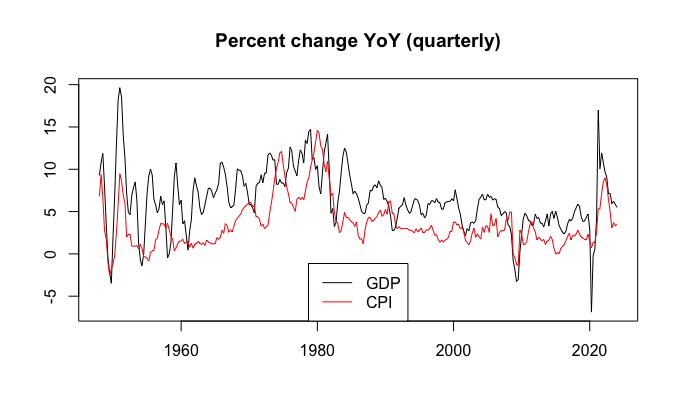
\includegraphics[width=0.75\linewidth]{INIT.png}
\end{figure}
The report begins by exploring basic \textbf{AR}, \textbf{MA} and \textbf{ARMA} models, then transitions to a more robust \textbf{VAR} specification to account interdependencies between the 2 variables. The model is fitted to the first 85\% of the data (training set), and predictive accuracy is evaluated on the remaining observations (test set). The methodology allows both in-sample reconstruction and out-of-sample forecasting, with uncertainty quantified via posterior credible intervals.

Visual diagnostics, posterior summaries, and prediction intervals support the evaluation of model adequacy. The results confirm the viability of Bayesian approaches in time series forecasting, especially when model flexibility and uncertainty quantification are key priorities. 
\newpage

\mainmatter
\chapter{Empirical Dataset Overview: US Quarterly GDP and CPI Time Series}
\label{ch:chapter_one}
\section{Preliminary Exploratory Analysis}
To evaluate the dynamic behavior of the time series, we compute and visualize their \textit{Autocorrelation Functions} (ACFs).
\subsubsection{GDP ACF}
\begin{itemize}
    \item The GDP series exhibits a strong spike at lag 1, followed by a slow decay with persistent positive autocorrelations across many lags.
    \item This behavior suggests non-stationarity and strong memory effects.
    The past information has a strong and persistent influence over time, meaning that current values in the series are highly dependent on a long sequence of past observations.
\end{itemize}
\begin{figure}[H]
    \centering
    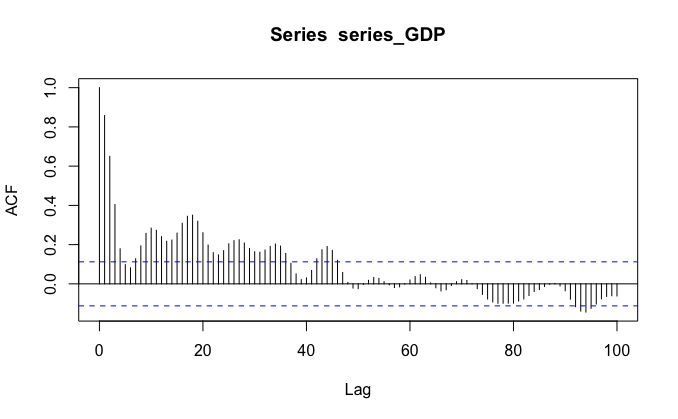
\includegraphics[width=0.80\linewidth]{GDP.png}
\end{figure}
\newpage
\subsubsection{CPI ACF}
\begin{itemize}
    \item The CPI series also shows very high autocorrelation at initial lags, but the decay is smoother and slower compared to GDP.
	\item The gradual decline of the autocorrelation function indicates that the series may possess long memory characteristics, where the effect of past shocks decays slowly but remains influential.
\end{itemize}
\begin{figure}[H]
    \centering
    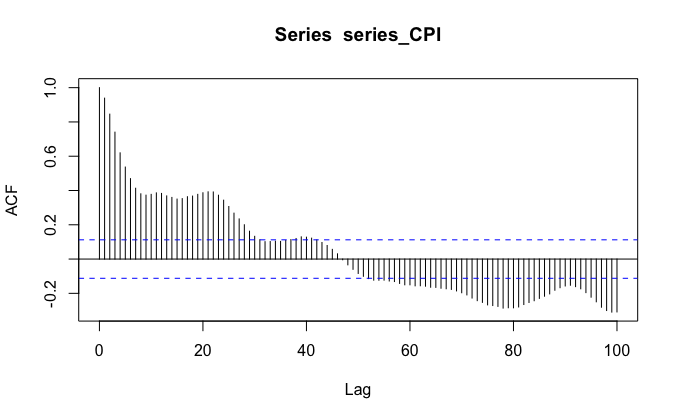
\includegraphics[width=0.80\linewidth]{CPI.png}
    \label{fig:enter-label}
\end{figure}

\section{Dataset Overview}
The original file \texttt{gdp\_inflation.csv} was pre-processed and aligned to guarantee a consistent length for both time series.
The seasonally adjusted indeces measure price changes (as a percent change) from the previous year. 
In order to rigorously assess the predictive capabilities of the proposed models, the dataset was judiciously partitioned into two disjoint subsets: a training set and a test set. 
\begin{itemize}
    \item The training set, comprising \textit{85\%} of the total observations, was employed to estimate the model parameters within a \textbf{Bayesian} framework.
    \item While the remaining \textit{15\%} the test set was reserved for the purpose of out-of-sample forecasting and model validation.
\end{itemize}
This temporal split not only ensures the integrity of the inference but also permits a realistic evaluation of the models’ forecasting performance on unseen data.

\chapter{Theoretical Foundations and Model Design in Time Series Inference}
\label{ch:chapter_two}
\subsection{Bayesian Modeling Rationale: Likelihood Construction and Prior Calibration}
\subsubsection{Likelihood: AR(n)}
Rather than writing a separate \texttt{JAGS block} for each autoregressive order, we defined one generic \textbf{\textit{AR(n)}} model string, where the order \textbf{\textit{n}} is simply passed in as a data argument.  This achieves two things:
\begin{itemize}
    \item \textbf{Flexibility}:  You can fit \textbf{\textit{AR(1)}}, \textbf{\textit{AR(2)}}, \textbf{\textit{AR(3)}}, … all in a single loop by varying the provided order parameter.
	\item \textbf{Maintainability}:  All future changes for example to the prior on the \textbf{\textit{AR}} coefficients need only be made once.
\end{itemize}

Recall that an AR(1) model is defined by
\begin{align}
y(t) &= a\,y(t-1) + \eta(t)\,, 
\quad \eta(t)\sim\mathcal{N}(0,\sigma^2)
\end{align}
Generalization of \textbf{\textit{AR(n)}}
\[
y(t) \;=\; \Bigl[\sum_{i=1}^{n}\alpha_i\,y(t-i)\Bigr]\;+\;\eta(t)
\qquad
\eta(t)\sim\mathcal{N}(0,\sigma^2)
\]
\begin{align}
y(t)
&=
\alpha_{1}\,y(t-1)
+ \alpha_{2}\,y(t-2)
+ \dots
+ \alpha_{n}\,y(t-n)
+ \eta(t)\,, 
\qquad
\eta(t)\sim\mathcal{N}(0,\sigma^2)
\end{align}
where $\alpha_{1},\dots,\alpha_{n}\in\mathbb{R}$.  In other words, it is simply a \emph{linear combination} of \(y(t)\) on its previous $n$ values, plus a noise.

\subsubsection{Prior of AR(n)}
\begin{itemize}
    \item \textbf{Intercept:} $m_0 \sim \mathcal{N}(0,10^4)$:\\
    Nearly flat Normal prior imparts almost no information on the mean level, letting the data dictate any non-zero drift.
    \item \textbf{Precision:} $\sigma^2 = \tau^{-1}, \quad \tau \sim \mathrm{Gamma}(0.1, 10)$:\\
    Gamma prior centers on a modest noise level while remaining diffuse enough to adapt to either low or hight variability, avoiding overconfidence in the error term. 
    \item \textbf{AR coefficient:} $\alpha_i \sim \mathcal{U}(-1.5,1.5)$:\\
    Uniform range slightly beyond $\pm 1$ allows the sampler to explore near unit root behavior (long memory) if supported by the data, yet still constrains extreme, implausible dynamics.
\end{itemize}


\subsubsection{Likelihood: MA(n)} 
We now define an \textbf{\textit{MA(1)}} (moving-average) process:
\begin{align}
y(t) &= \alpha\,\eta(t-1) + \eta(t)\,, 
\quad \eta(t)\sim\mathcal{N}(0,\sigma^2)\,
\end{align}
  
An \textbf{\textit{MA(1)}} captures serial correlation by linearly combining the current white-noise shock \(\eta(t)\) with the immediately preceding shock \(\eta(t-1)\).  
Such a model is particularly useful in time series analysis when short term dependencies (one lag) dominate and higher order moving averages add little explanatory power.\\
As with the \textbf{\textit{AR}} case, we defined a generic JAGS implementation for the \textbf{\textit{MA(n)}} process, enabling flexible evaluation across different orders by simply adjusting the lag parameter.
\subsubsection{Prior of MA(1)}
\begin{itemize}
    \item \textbf{Intercept:} $m_0 \sim \mathcal{N}(0,10^4)$\\
    An almost flat Normal prior that leaves the series mean entirely data-driven.
    \item \textbf{Precision:} $\tau \sim \mathrm{Gamma}(0.01,0.01)$\\
    Highly diffuse Gamma prior on the noise precision, accommodating both low and high variance regimes.
    \item \textbf{MA coefficient:} $
\beta \sim \mathcal{N}\left(0, 10 \right)
$\\
Normal prior on MA coefficients introduces slight shrinkage toward zero, offering a more regularized alternative to the uniform prior while preserving flexibility in capturing short-term shocks.

\end{itemize}


\subsubsection{Likelihood: ARMA(1,1)}
After having explored both auto-regressive and moving average components independently, we now propose a more comprehensive model that integrates both effects: the ARMA(1,1) process. This specification combines the dynamics of $AR(1)$ and $MA(1)$ structures into a single model, capturing both short-term memory and random shock propagation. The model is expressed as follows:

\begin{equation}
y(t) = \alpha\, y(t-1) + \beta\, \eta(t-1) + \eta(t), \qquad \eta(t) \sim \mathcal{N}(0, \sigma^2)
\end{equation}
where $\alpha$ governs the persistence of the process and $\beta$ controls the contribution of the previous white noise term. This formulation allows the model to capture both autoregressive dynamics and noise-driven volatility.

The motivation for selecting an \textbf{\textit{ARMA(p,q)}} model arises from the observation that higher-order autoregressive models (i.e., $AR(n)$ with $n > 1$) did not yield significant improvement in predictive accuracy. On the contrary, model comparison metrics (such as \textbf{WAIC}) suggested that a deeper memory structure was sufficient to capture the temporal dependencies in our dataset. The \textbf{\textit{ARMA(p,q)}} model thus provides a parsimonious yet effective trade-off between model complexity and explanatory power.
\subsubsection{Prior of ARMA(p,q)}
\begin{itemize}
    \item \textbf{Intercept:} $m_0 \sim \mathcal{N}(0,10^4)$\\
    An almost flat Normal prior that leaves the series mean entirely data-driven.
    \item \textbf{AR coefficient:}  
    $\alpha \sim \mathcal{U}(-1.5,1.5)$\\
    Uniform prior enforcing the invertibility condition while remaining non-informative about the MA effect.
    \item \textbf{MA coefficient:}  
     $\beta \sim \mathcal{N}\left(0, 10 \right)$\\
    Normal priors on ARMA coefficients provide mild regularization while allowing flexible dynamics.
    \item \textbf{Noise precision:}  
    $\tau \sim \mathrm{Gamma}(0.01,0.01)$\\
    Highly diffuse Gamma prior on the error precision, accommodating both low and high noise regimes.
    
\end{itemize}
\subsubsection{Likelihood: VAR(n)}
To enrich the inferential scope of our analysis, we extend the univariate time series approach by jointly modeling the \textbf{U.S. GDP} growth and inflation dynamics through a \textbf{Vector Autoregressive} model \textbf{\textit{VAR(n)}}. Unlike separate univariate models, a \textbf{\textit{VAR}} framework allows us to account for contemporaneous feedback and temporal interdependencies between multiple economic indicators.

The model is specified as:
\[
{y}_t
\;=\;
\sum_{o=1}^{p} A_{o}\,y_{t-o}
\;+\;
m_{0}
\;+\;
\varepsilon_t,
\qquad
\varepsilon_t \sim \mathcal{N}\bigl(0,\Sigma)
\]
%\paragraph{Difference between AR and VAR models:}
%-> TODO: Spiegazione delle differenze fra AR e VAR, e cosa ci aspettiamo di vedere all'interno della predizione
%In the \textbf{\textit{AR}} model, a single variable is analyzed over time: each future value is predicted based on the past values of that same variable. In other words, the evolution of the series is assumed to depend only on itself. One the other hand, the \textbf{\textit{VAR}} model consider multiple variables simultaneously: each one is explained by its own past values as well as those of the others. This approach is particularly useful when studying the dynamic relationship between economic varibales that influence each other, such as \textbf{GDP} and \textbf{Infaltion}.
%Far notare le differenze con AR models alla luce dei risultati trovati all'interno delle metriche di valutazione%

\subsubsection{Prior of VAR(n)}
\begin{itemize}
    \item \textbf{Transition coefficients:}  
    $A_{i,j,o} \sim \mathcal{N}(0,\,10)$\\
    Weakly informative Normal prior centered at zero with variabce 0.1, gently shrinking cross-variable effect while allowing moderate dynamic interactions.
    \item \textbf{Innovation precision matrix:}  
    $\boldsymbol{\tau} \sim \mathrm{Wishart}(I,\,3),\;\boldsymbol{\Sigma}=\boldsymbol{\tau}^{-1}$\\
    Conjugate Wishart prior with scale \(I\) and minimal degrees of freedom \(\nu=3\), yielding a diffuse yet proper prior over the $\text{\itshape 2}\!\times\!\text{\itshape 2}$ covariance.
    \item \textbf{Intercept vector:}  
    $m_{\text{gdp}},\,m_{\text{infl}} \sim \mathcal{N}(0,\,10^4),\;\mathbf{m}_0=\begin{pmatrix}m_{\text{gdp}}\\m_{\text{infl}}\end{pmatrix}$\\
    Nearly flat Normal priors on each intercept component, ensuring the long-run means are driven by the data.
\end{itemize}
The others priors that we use during our comparison are specified significantly at \ref{Prior-VAR}.

\chapter{Bayesian Blueprint: Prior Beliefs and Model Structure}
%TODO:  Risultati e confronto\\
 %-> Grafici: boxplot o barplot.\\
 %-> Forecast vs. dati reali (Test-Set): ¿due figure (una per serie) con intervalli di confidenza?\\
%-> Trace-Plot\\
%-> Validation Set\\
%\sout{---> SUDDIVISIONE GPD-CPI IN 2 SEZIONI SEPARATE}\\
We now begin our discussion aimed at understanding the temporal dynamics within the \textbf{GDP} and, subsequently, \textbf{CPI} datasets through the application of \textbf{\textit{AR}}, \textbf{\textit{MA}}, \textbf{\textit{ARMA}}, and \textbf{\textit{VAR}} models. Our journey into the deeper structure of these models will unfold in two distinct stages: we will start with the analysis of \textbf{GDP}, followed by that of \textbf{CPI}.
In this section, we present time series plots along with a discussion justifying the selected parameter values. We conclude with a brief qualitative comment on the observed dynamics.\\

The next chapter will focus on model comparison using several evaluation criteria, including both complexity-penalized metrics and prediction accuracy scores:
\begin{itemize}
    \item \textbf{DIC} (Deviance Information Criterion),
    \item \textbf{WAIC} (Watanabe–Akaike Information Criterion),
    \item \textbf{BIC} (Bayesian Information Criterion),
    \item Classical test error metrics (on unseen data) metrics such as:
    \begin{itemize}
  \item \textbf{MSE} (Mean Squared Error)
  \item \textbf{MAE} (Mean Absolute Error)
  \item \textbf{MAPE} (Mean Absolute Percentage Error)
  \item \textbf{SMAPE} (Symmetric Mean Absolute Percentage Error)
  \item \textbf{MASE} (Mean Absolute Scaled Error)
    \end{itemize}
\end{itemize}
These indicators allow us to quantify both model fit and out-of-sample predictive accuracy.

\subsection{Legend for Interpretation}
In order to guide the reader toward a robust and informed interpretation of the graphical evidence presented, we provide below the essential keys to correctly decode the underlying dynamics.

\begin{table}[H]
  \centering
  \setlength\tabcolsep{8pt}
  \renewcommand{\arraystretch}{1.2}
  \fbox{%
    \begin{tabular}{@{} ll @{}}
      \multicolumn{2}{c}{\textbf{Legend}} \\[4pt]
      \textcolor{red}{\rule{1cm}{1pt}} 
        & Observed data \\
      \textcolor{blue}{\raisebox{0.5ex}{\textasteriskcentered}} 
        & In-sample predictions (mean) \\
      \textcolor{blue}{\rule{1cm}{1pt}} 
        & 95\% credible interval (in-sample) \\
      \textcolor{orange}{\raisebox{0.5ex}{\textasteriskcentered}} 
        & Out-of-sample forecasts (mean) \\
      \textcolor{orange}{\rule{1cm}{1pt}} 
        & 95\% credible interval (out-of-sample) \\
      \textcolor{orange}{\tikz{\draw[orange,dashed, line width=0.8pt] (0,0)--(1cm,0);}} 
        & 50\% credible interval (out-of-sample) \\
      \textcolor{magenta}{\tikz{\draw[magenta, line width=1pt] (0,0)--(0,0.8cm);}} 
        & End of training set \\
      \textcolor{green}{\rule{1cm}{1pt}} 
        & Posterior mean of $m_{0}$ \\
    \end{tabular}%
  }
\end{table}
\begin{itemize}
  \item \textbf{Full-range plot (in-sample + out-of-sample)}\\
  The first panel illustrates the entire time series dynamics. The observed data are shown in \textcolor{red}{red}, over which the following elements are superimposed:
  \begin{itemize}
    \item \textit{In-sample predictions}, plotted as blue asterisks, accompanied by \texttt{\textbf{95\% credible intervals}} represented by \textcolor{blue}{----- solid blue} lines connecting the \texttt{2.5\%} and \texttt{97.5\% quantiles}.
    \item \textit{Out-of-sample forecasts}, plotted as \textcolor{orange}{* orange asterisks}, with:
    \begin{itemize}
      \item \texttt{\textbf{95\% credible bands}}: \textcolor{orange}{----- solid orange} lines between the \texttt{2.5\%} and \texttt{97.5\% quantiles};
      \item \texttt{\textbf{50\% credible bands}}: dashed \textcolor{orange}{- - - - dashed orange} lines between the \texttt{25\%} and \texttt{75\% quantiles} .
    \end{itemize}
    \item A \textcolor{magenta}{| dashed magenta} vertical line marks the end of the training set, clearly separating the in-sample from the out-of-sample region.
    \item A \textcolor{green}{- - - dashed green} horizontal line represents the posterior mean estimate of $m_0$, i.e., the average level of the series as inferred by the model.
  \end{itemize}

  \item \textbf{Zoom on the out-of-sample forecast}\\
  The second panel zooms into the last $K$ training observations (default: $K=5$) and the entire out-of-sample interval. Again:
  \begin{itemize}
    \item The real series is plotted in \textcolor{red}{red};
    \item The same \textcolor{magenta}{magenta} and \textcolor{green}{green} reference lines are maintained;
    \item The out-of-sample forecasts and their associated \texttt{\textbf{95\%}} and \texttt{\textbf{50\%} credible intervals} are shown as in the previous panel, providing a more focused view on predictive performance.
  \end{itemize}
\end{itemize}

This two-panel visualisation allows for a comprehensive assessment of the model's fit to historical data and the reliability of future projections. The overlap between observed and predicted values enables immediate visual comparison, highlighting both the pointwise accuracy and the uncertainty estimated by the model.
%Iniziamo ora la nostra trattazione dedicata alla comprensione delle dinamiche temporali contenute nei dataset di GDP e, successivamente, di CPI, attraverso l’applicazione dei modelli AR, MA, ARMA e VAR. Il nostro viaggio all’interno dei meandri più profondi di queste strutture avverrà in due tappe distinte: inizieremo con l’analisi del GDP per poi passare al CPI. Abbiamo scelto questa sequenza per favorire una lettura più fluida e una comprensione progressiva dei risultati. In questa sezione saranno presentati i grafici relativi alle serie temporali, accompagnati da un’analisi delle motivazioni che ci hanno portato a selezionare determinati valori dei parametri stimati. Concluderemo con un breve commento qualitativo sull’andamento della dinamica osservata.
%Nel capitolo successivo ci concentreremo invece sulla valutazione comparativa dei modelli tramite diverse metriche di accuratezza e complessità, tra cui:
%DIC (Deviance Information Criterion),
%WAIC (Watanabe–Akaike Information Criterion),
%BIC (Bayesian Information Criterion),
%e misure di errore predittivo quali MSE, MAE, MAPE, SMAPE, MASE.
%Queste ultime ci permetteranno di quantificare la bontà del fit e la capacità di previsione out-of-sample.


%A questo punto volgliamo togliere anche "price"? Va bene
%Si si togliamoli, infatti di solito la descrizione non la metto mai. Ho fatto un file pages che devo ricontrollare dove ho scritto tutta la descrizione delle serie ecc ed i relativi confronti fra i diversi modelli. Aggiungo che sarà presente una versione in-sample+oos e una solomente con oos zoomata

% Si, direi di si, tanto si dovrebbe capire

% Forse toglierei anche quei (a) FMA(1) ... (b) ZMA(1), perchè in parte l'ordine c'è scritto sopra a ogni grafico, e il fatto che uno è tutta la serie e l'altra è la versione zoommata lo possiamo scrivere nel "Figure 3.1: MA(1) and MA(4) fits (full series and zoomed out-of-sample prediction)

% ci sta
%->TODO: AGGIUNGI TESTO DESCRIZIONE MODELLI FILE PAGES
%\subsection{Structural Patterns in Quarterly GDP: An Empirical Time Series Investigation}
\newgeometry{left=1cm,right=1cm}  % <-- pick whatever you like
\subsubsection{GDP Dynamics under AR Modeling}
%Nella seguente sezione analizzeremo il modello AR.
\begin{figure}[H]
  \centering
  \begin{tabular}{@{}cc@{}}
    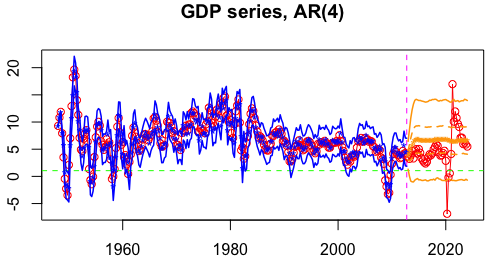
\includegraphics[angle=90,width=0.33\linewidth]{FAR(4)-1.png} &
    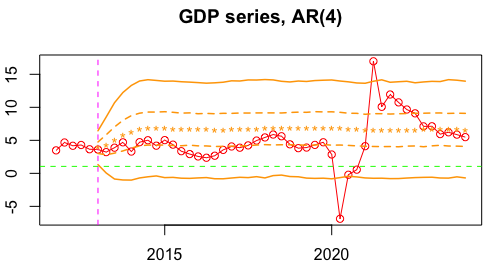
\includegraphics[angle=90,width=0.33\linewidth]{ZAR(4)-1.png} \\
    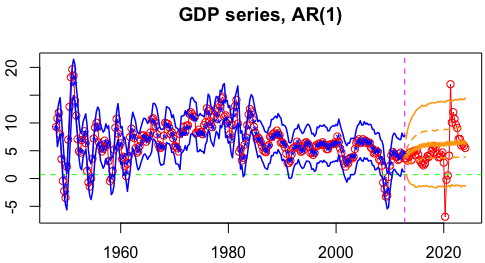
\includegraphics[angle=90,width=0.33\linewidth]{FAR(1)-2.png} &
    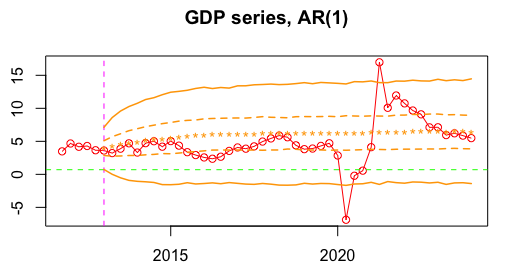
\includegraphics[angle=90,width=0.335\linewidth]{ZAR(1)-1.png}
  \end{tabular}
\end{figure}
\restoregeometry

\subsection*{Comparison of AR(1) and AR(4)}
From the analysis of the plots in the figure, two clearly distinct behaviors emerge. The \textbf{\textit{AR(1)}} model, while being extremely responsive to the most recent movements, struggles to capture medium-term oscillations, which is reflected in wider uncertainty bands (yellow lines) immediately after the training/test split.


In contrast, the \textbf{\textit{AR(4)}} model incorporates information over a longer horizon, that is, the observed values of the time series in the four previous time points, absorbing peaks and drops more gradually: the forecast trajectory is smoother and the uncertainty bands are overall narrower in the out-of-sample. 

In this way, the \textbf{\textit{AR(4)}} provides a less volatile forecast, although at the cost of a more delayed response to recent shocks. These elements suggest that, for our quarterly \textbf{U.S. GDP dataset}, an intermediate order (such as 4) represents a good compromise between responsiveness and stability of the forecasts.



\subsubsection{GDP Dynamics under MA Modeling}
%\quad{->TODO: DA QUA MODIFICARE I PLOT RIMUOVENDO "time" e "price"}

%{AREASMA-GDP.png} 
%{TraceMA-GDP.png}

\begin{figure}[H]
  \centering
  \begin{tabular}{@{}cc@{}}
    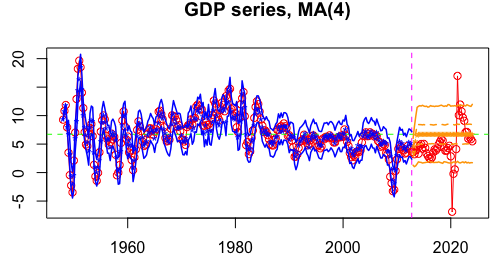
\includegraphics[angle=90,width=0.33\linewidth]{FMA(4)-1.png} &
    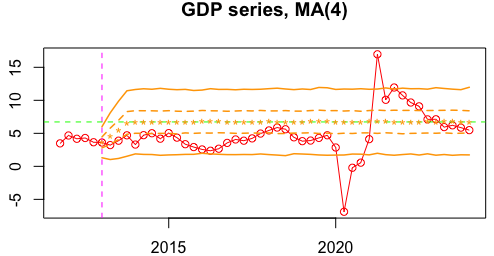
\includegraphics[angle=90,width=0.33\linewidth]{ZMA(4)-1.png} \\
    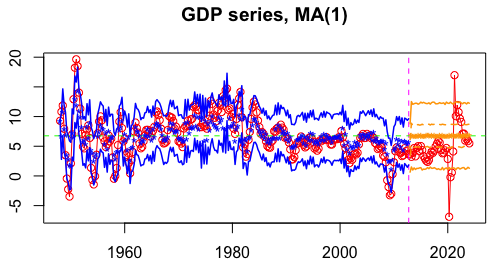
\includegraphics[angle=90,width=0.33\linewidth]{FMA(1)-1.png} &
    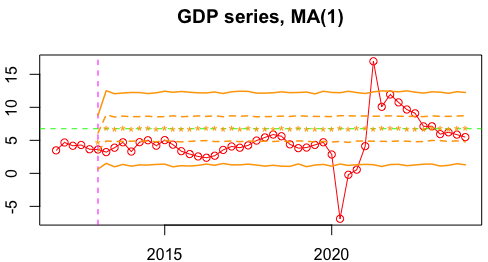
\includegraphics[angle=90,width=0.335\linewidth]{ZMA(1)-1.png}
  \end{tabular}
\end{figure}

\newpage
\subsubsection*{Comparison of MA(1) and MA(4)}
 From this comparison we observe:

\begin{itemize}
  \item \textbf{\textit{MA(1)}} relies solely on the single most recent residual, producing highly \emph{reactive} forecasts: its out-of-sample uncertainty band is wide and adjusts immediately to the last training point’s fluctuation.
  \item \textbf{\textit{MA(4)}}, by incorporating the four latest residuals, yields \emph{smoothed} predictions: its point forecasts fluctuate less and its credibility intervals narrow, indicating greater stability at the cost of a slower response to abrupt shocks.
\end{itemize}

In essence, \textbf{\textit{MA(4)}} averages extreme events over several past lags dampening, their influence on future predictions, whereas \textbf{\textit{MA(1)}} reflects each recent spike directly in its forecast.

\bigskip

%\subsubsection*{Traceplots and Posterior Densities of \(\beta\) and \(m_0\)}

%Alongside the forecast plots, we examine key MCMC diagnostics:

%\begin{description}
  %\item[Traceplots] depict the sampled trajectories of \(\beta\) and \(m_0\) across iterations. Ideal traceplots resemble a \textit{“fat hairy caterpillar”} with no visible trend, signaling rapid convergence to stationarity and thorough exploration of the posterior support without getting trapped in local modes.
  %\item[Density plots] show the estimated posterior distributions of \(\beta\) and \(m_0\) after burn-in. In our analysis, \(\beta\)’s density is tightly concentrated around its estimated value, while \(m_0\) confirms a stable central level with low dispersion.
%\end{description}

%Together, these diagnostics validate the convergence and robustness of our parameter estimates, bolstering confidence in the resulting forecasts.


\subsubsection{GDP Dynamics under ARMA Modeling}

\begin{figure}[H]
  \centering
  \begin{tabular}{@{}ccc@{}}
    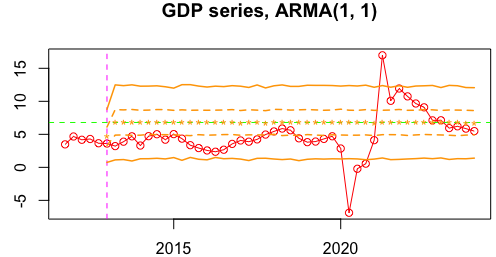
\includegraphics[angle=90,width=0.3\linewidth]{ZARMA(1,1)-1.png} &
    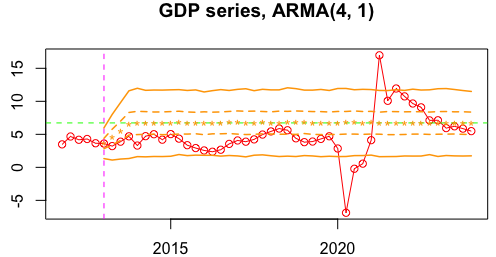
\includegraphics[angle=90,width=0.302\linewidth]{ZARMA(4,1)-1.png} &
    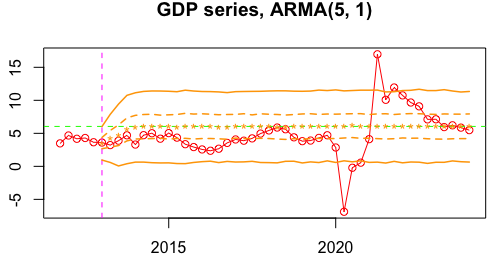
\includegraphics[angle=90,width=0.305\linewidth]{ZARMA(5,1)-1.png} \\
    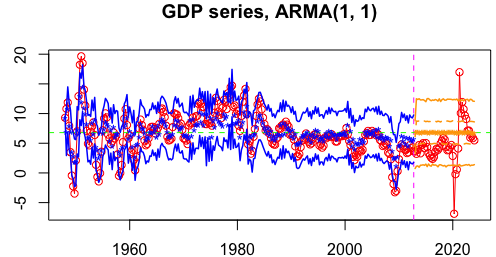
\includegraphics[angle=90,width=0.3\linewidth]{FARMA(1,1)-1.png} &
    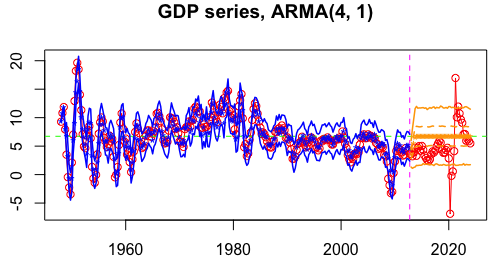
\includegraphics[angle=90,width=0.3\linewidth]{FARMA(4,1)-1.png} &
    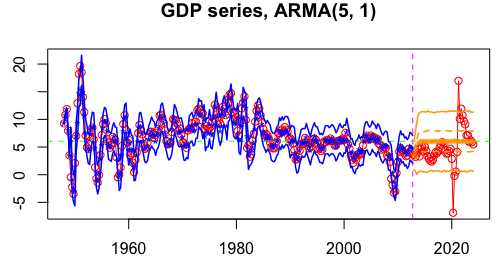
\includegraphics[angle=90,width=0.29\linewidth]{FARMA(5,1)-1.png}
  \end{tabular}
  % \caption{Visual comparison of MA(1) and MA(4) model fits and diagnostic plots.}
  % \label{fig:MA_models}
\end{figure}
\newpage
\subsubsection*{Comparison of ARMA(1,1), ARMA(4,1), ARMA(5,1)}
In describing the dynamics of the \textbf{GDP} via ARMA models, the interplay between autoregressive and moving‐average terms becomes immediately apparent. The \textbf{\textit{ARMA(1,1)}} model tracks very recent fluctuations with remarkable agility thanks to its single lag AR component but this narrow horizon comes at the cost of notably wider credible bands as soon as one moves beyond the training sample. 

By extending the autoregressive order to four lags, as in \textbf{\textit{ARMA(4,1)}}, we achieve a smoothing effect: peaks and troughs are absorbed more gradually, the forecast path appears more polished, and the credibility intervals tighten considerably, yielding greater stability without sacrificing responsiveness. Pushing further to \textbf{\textit{ARMA(5,1)}} offers only marginal gains, indicating that beyond a certain point additional lags provide diminishing returns. 

Ultimately, for our quarterly \textbf{U.S GDP} sample, the \textbf{\textit{ARMA(4,1)}} specification strikes the best balance: it “remembers” medium‐term oscillations while still adapting promptly to recent shocks, and it delivers overall narrower uncertainty bands.  

\subsubsection{CPI Dynamics under AR Modeling}
\begin{figure}[H]
  \centering
  \begin{tabular}{@{}cc@{}}
    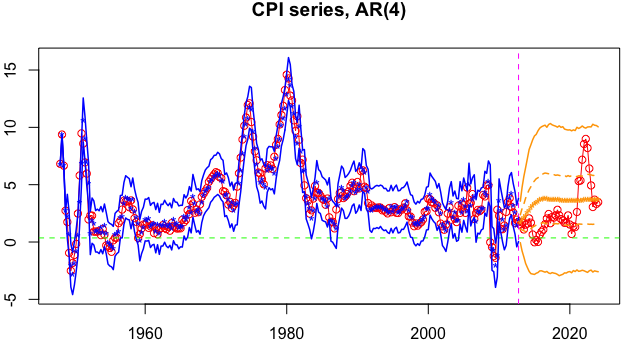
\includegraphics[angle=90,width=0.33\linewidth]{CPI_FAR(4).png} &
    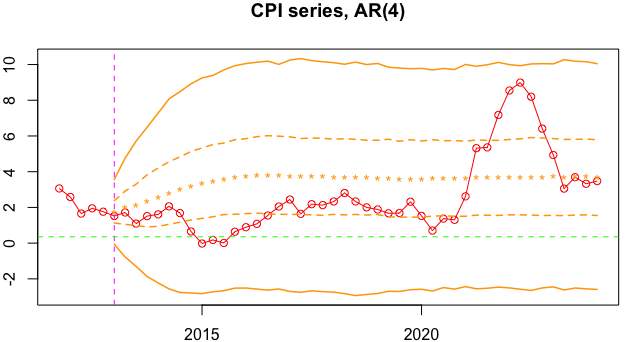
\includegraphics[angle=90,width=0.33\linewidth]{CPI_ZAR(4).png} \\
    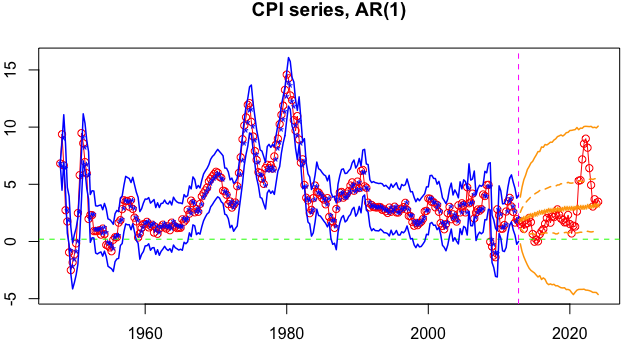
\includegraphics[angle=90,width=0.33\linewidth]{CPI_FAR(1).png} &
    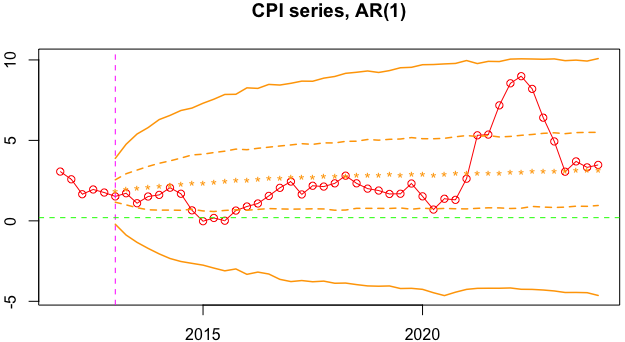
\includegraphics[angle=90,width=0.335\linewidth]{CPI_ZAR(1).png}
  \end{tabular}
\end{figure}


\subsubsection*{Comparison of AR(1) and AR(4)}
For the \textbf{CPI}, the comparison between \textbf{AR(1)} and \textbf{AR(4)} reveals dynamics analogous to those observed for the \textbf{GDP}, but on a more pronounced price‐change scale:
\begin{itemize}
    \item The \textbf{\textit{AR(1)}} model reacts very quickly to the most recent monthly inflation swings, yet produces relatively wide uncertainty bands beyond the training window, since it “forgets” all but the last observation.
	\item The \textbf{\textit{AR(4)}} model incorporates information from the past four months, naturally smoothing sharp spikes and tightening the out-of-sample credible intervals. The result is a more stable forecast that still retains reasonable responsiveness to inflation peaks.
\end{itemize}


Overall, even for the \textbf{CPI}, an intermediate lag order (\textbf{4}) offers an effective balance: it captures short-term movements without unduly inflating forecast uncertainty.

\subsubsection{CPI Dynamics under MA Modeling}

\begin{figure}[H]
  \centering
  \begin{tabular}{@{}cc@{}}
    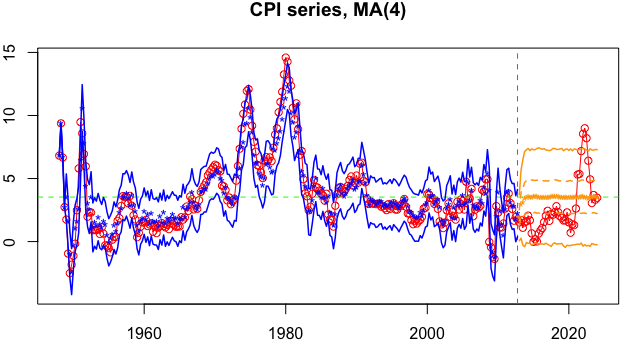
\includegraphics[angle=90,width=0.33\linewidth]{CPI_FMA(4).png} &
    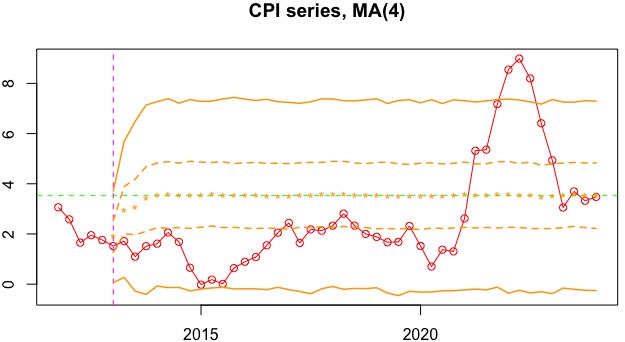
\includegraphics[angle=90,width=0.33\linewidth]{CPI_ZMA(4).png} \\
    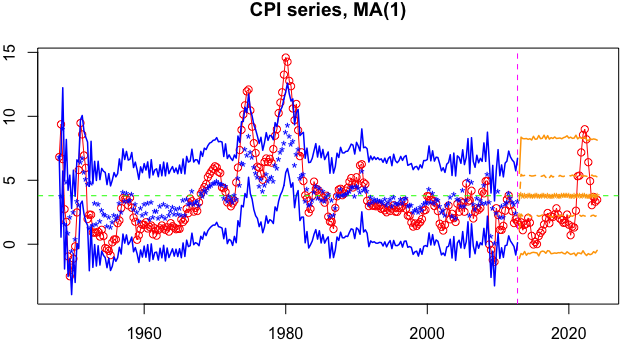
\includegraphics[angle=90,width=0.33\linewidth]{CPI_FMA(1).png} &
    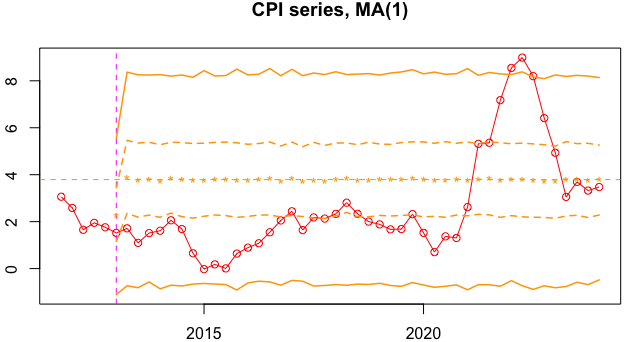
\includegraphics[angle=90,width=0.335\linewidth]{CPI_ZMA(1).png}
  \end{tabular}
\end{figure}
\newpage
\subsubsection*{Comparison of MA(1) and MA(4)}

In these panels we compare two moving-average specifications applied to the \textbf{CPI} series:
\begin{itemize}
  \item \textbf{\textit{MA(1)}} relies on a single past innovation, yielding high sensitivity to monthly spikes but relatively wide out-of-sample credible bands.
  \item \textbf{\textit{MA(4)}} incorporates the four most recent residuals, which smooths abrupt jumps and tightens the credible intervals, resulting in more stable forecasts while still accommodating short-term shocks.
\end{itemize}

Overall, even for the \textbf{CPI}, an intermediate lag order (\textbf{4}) strikes an effective balance between responsiveness and forecast precision.



\subsubsection{CPI Dynamics under ARMA Modeling}

\begin{figure}[H]
  \centering
  \begin{tabular}{@{}ccc@{}}
    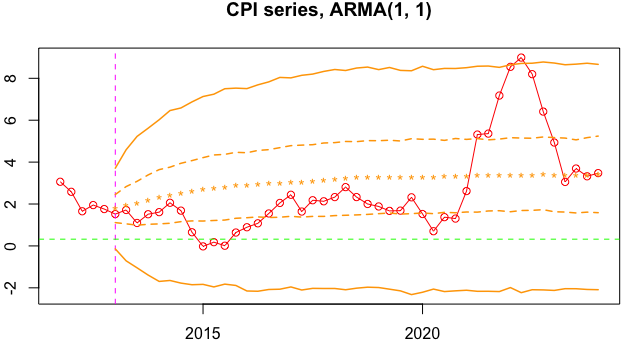
\includegraphics[angle=90,width=0.3\linewidth]{CPI_ZARMA(1,1).png} &
    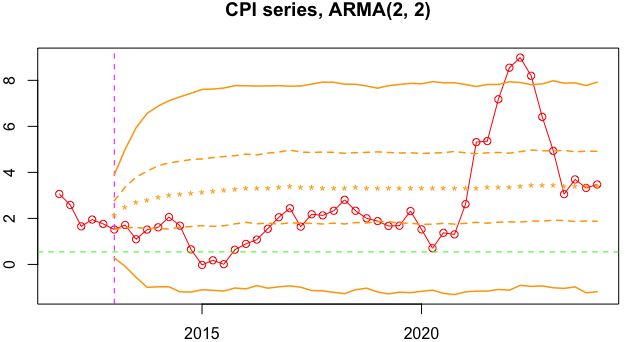
\includegraphics[angle=90,width=0.302\linewidth]{CPI_ZARMA(2,2).png} &
    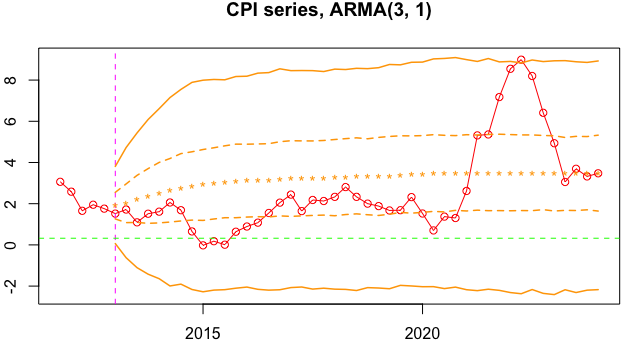
\includegraphics[angle=90,width=0.305\linewidth]{CPI_ZARMA(3,1).png} \\
    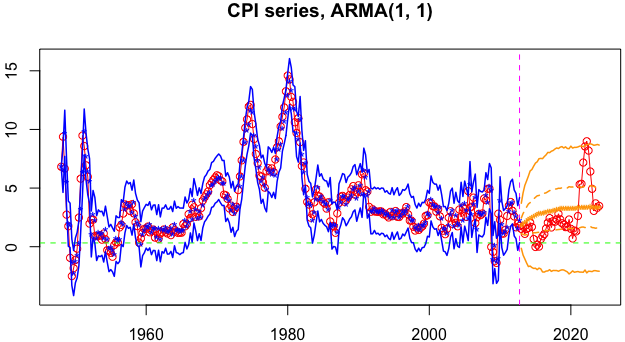
\includegraphics[angle=90,width=0.3\linewidth]{CPI_FARMA(1,1).png} &
    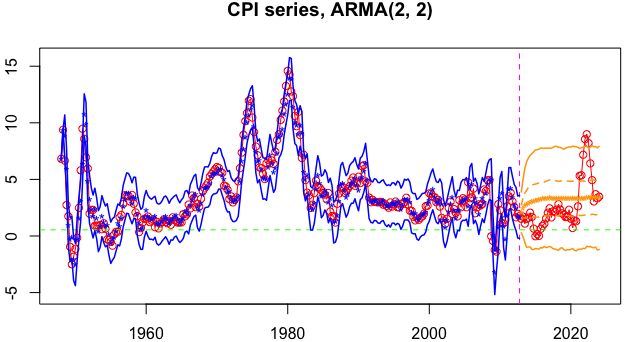
\includegraphics[angle=90,width=0.3\linewidth]{CPI_FARMA(2,2).png} &
    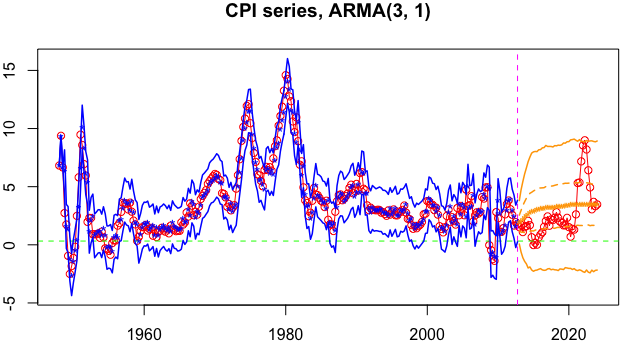
\includegraphics[angle=90,width=0.29\linewidth]{CPI_FARMA(3,1).png}
  \end{tabular}
  % \caption{Visual comparison of MA(1) and MA(4) model fits and diagnostic plots.}
  % \label{fig:MA_models}
\end{figure}
\newpage
\subsubsection*{Comparison of ARMA(1,1), ARMA(4,1), ARMA(5,1)}
In the panels below we compare the in-sample fit and out-of-sample forecasts for three \textbf{\textit{ARMA}} specifications applied to the \textbf{CPI} series:
\begin{itemize}
  \item \textbf{\textit{ARMA(1,1)}} combines one autoregressive lag and one moving-average term, achieving high sensitivity to recent fluctuations but relatively wide credible bands immediately after the training/test split.
  \item \textbf{\textit{ARMA(2,2)}} incorporates two lags in both AR and MA components, better capturing both short and medium-term oscillations and yielding somewhat tighter credible intervals.
  \item \textbf{\textit{ARMA(3,1)}} uses three autoregressive lags with a single MA term, providing an intermediate profile that balances responsiveness and stability in the forecast trajectory.
\end{itemize}

Overall, the choice of lag orders governs the trade-off between rapid shock absorption and uncertainty compression: for our quarterly \textbf{CPI} sample, an intermediate specification such as \textbf{\textit{ARMA(2,2)}} appears to deliver the most balanced performance.
\newpage

\subsubsection{GDP-CPI Dynamics under VAR Modeling}
\begin{figure}[H]
  \centering
  \begin{tabular}{@{}cc@{}}
    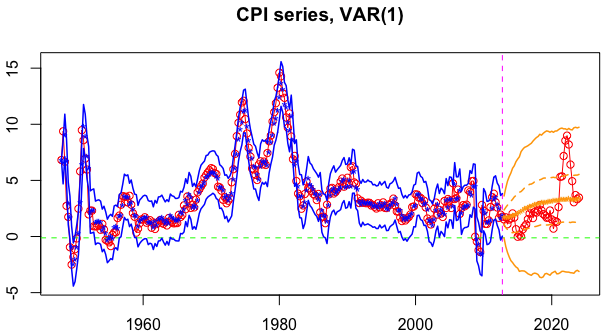
\includegraphics[angle=90,width=0.35\linewidth]{VAR(1)-33.png} &
    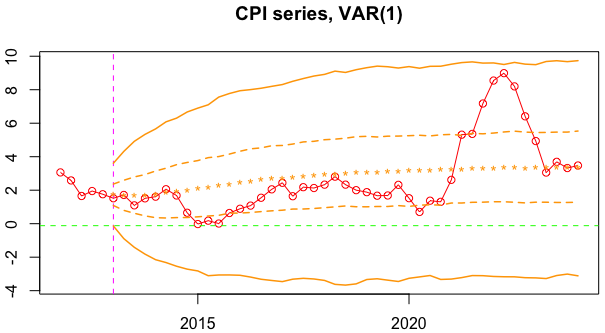
\includegraphics[angle=90,width=0.35\linewidth]{VAR(1)-44.png} \\
    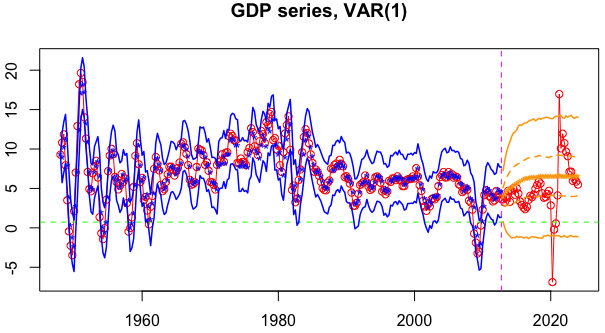
\includegraphics[angle=90,width=0.35\linewidth]{VAR(1)-11.png} &
    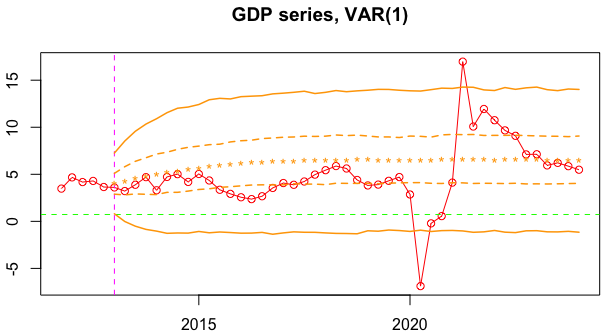
\includegraphics[angle=90,width=0.35\linewidth]{VAR(1)-22.png}
  \end{tabular}
\end{figure}



\subsection*{Assessment of Contemporaneous Correlation through Prior Specification}

The objective of our analysis is to determine whether a certain degree of correlation exists between the respective stochastic components of the two time series. To formally investigate the residuals estimated under a \textbf{\textbf{Wishart}} prior for the \textbf{GDP} and \textbf{CPI} series, we compute the \textit{Pearson} correlation coefficient, which allows us to quantify the strength and direction of the linear relationship between the errors of two macroeconomic variables.
\label{Prior-VAR}
\paragraph{Case 1: Diagonal Prior (Uncorrelated Errors)}
Our empirical exploration will initially focus on the deliberate choice of a diagonal prior in order to impose a zero-correlation structure between the residuals of \textbf{GDP} and \textbf{CPI}. 

Consequently, given the absence of non-zero entries outside the diagonal in the precision matrix (i.e., non-zero values only along the diagonal), we enforce the assumption of no correlation between the two variables. In doing so, we model a dynamic in which shocks affect only the series to which they belong, thereby enabling a meaningful comparison with the alternative hypothesis of correlated errors, which will be addressed through the specification of a \textit{Wishart} prior.
\[
\tau =
\begin{pmatrix}
\tau_{11} & 0 \\
0 & \tau_{22}
\end{pmatrix}, 
\quad \text{with} \quad
\tau_{11}, \tau_{22} \sim \text{Gamma}(a, b).
\]

\paragraph{Case 2: Wishart Prior (Correlated Errors)}
In contrast, by adopting a \textbf{Wishart} prior, we allow the covariance between the residuals to be freely estimated. Accordingly, we define a precision matrix with non-zero entries outside the diagonal, as long as it remains positive definite, i.e., invertible and allowing the density to be well-defined. In this way, the model is able to estimate the strength of the correlation between \textbf{\textit{GDP}} and \textbf{\textit{CPI}} directly from the data. 
\[
\tau \sim \text{Wishart}(R, 3), \quad \text{where} \quad
R = \begin{pmatrix}
1 & 0 \\
0 & 1
\end{pmatrix}.
\]

This enables estimation of the off-diagonal covariance terms directly from the data.

\newpage

\textbf{Posterior Means}\\

\textbf{Using Diagonal Prior:}
\[
A =
\begin{pmatrix}
0.9085 & -0.0350 \\
0.0801 & \phantom{-}0.8854
\end{pmatrix}, \quad
\sigma^2 =
\begin{pmatrix}
2.6105 & 0 \\
0 & 0.9590
\end{pmatrix}
\]

\textbf{Using Wishart Prior:}
\[
A =
\begin{pmatrix}
0.9083 & -0.0364 \\
0.0795 & \phantom{-}0.8854
\end{pmatrix}, \quad
\sigma^2 =
\begin{pmatrix}
2.5838 & 0.5505 \\
0.5505 & 0.9538
\end{pmatrix}
\]

\paragraph{Empirical Results}
The \textit{Pearson} correlation coefficient between the residuals obtained from the model with a Wishart prior is:
\[
\rho(\text{err}_{\mathrm{GDP}},\,\text{err}_{\mathrm{CPI}}) 
= \frac{\text{Cov}(\text{err}_{\mathrm{GDP}}, \text{err}_{\mathrm{CPI}})}{
\sqrt{\text{Var}(\text{err}_{\mathrm{GDP}}) \cdot \text{Var}(\text{err}_{\mathrm{CPI}})}} 
= \frac{0.5505}{\sqrt{2.5838 \cdot 0.9538}} \approx 0.3507.
\]
Based on the result of the \textit{Pearson} correlation coefficient which allows us to check whether it is reasonable to assume correlation between the residuals and to quantify its intensity we can conclude that a value of approximately \texttt{0.35} represents a moderate and positive correlation.

The correlation is not null, yet not dominant either: it improves, albeit slightly, the modeling of contemporaneous volatility, but it does not affect the lagged dynamics—indeed, the matrix \textit{A} remains nearly unchanged.

We specified these priors for the \textbf{\textit{VAR}} because, in sensitivity checks using alternative prior formulations, the estimated dynamic relationships did not change significantly.

\chapter{Metrics of Truth: Evaluating Models Beyond the Horizon}
\subsection{Performance Assessment of Univariate Time Series}
\textbf{Performance comparison across AR, MA, and ARMA models on evaluation metrics. Best results in each block are highlighted in bold.}

%TRADUCI: Affronteremo ora una delicata valutazione sulla natura e bontà delle nostre analisi sulla base di metriche che ci possono aiutare nella più difficile scelta dell'ideale famiglia di modelli e della relativa parametrizzazione che rappresenta e prevede al meglio la dinamica dei nostri indicatori GDP e CPI. Procederemo poi con una disamina più approfondita, strutturata sulla scelta ideale del modello, non solamente corroborata da analisi matematiche ma qualcosa che sarà frutto anche di un' indagine squisitamente empirica.  
%Come possiamo notare dalle due tabelle sono rappresentati a livello di colonne le varie metriche di valutazione e sulle righe sono posizionati (suddivisi nelle diverse model-family) i modelli con la relativa parametrizzazione. 
%Nota importante: il modello BIC sarà prevalentemente il nostro modello di riferimento, secondo la nostra analisi è quello che meglio incorpora la valutazione del modello out-of-sample poichè ci permette di ponderare al meglio la sensibilità dell’andamento dei dati con la complessità del modello. 
%Successivamente nella nostra trattazione affronteremo anche grafici quali Trace plot, Density plot e Interval plot.
We will now undertake a rigorous assessment of the validity and effectiveness of our analyses by means of a suite of evaluation metrics designed to guide the challenging task of identifying which specific model or entire model family and its parametrization best capture and forecast the dynamics of our \textbf{GDP} and \textbf{CPI} indicators.

We will then move on to a deeper examination of the ideal model choice, one that is supported not only by formal mathematical criteria but also by a thoroughly empirical investigation.


As shown in the two tables, each column corresponds to a distinct evaluation metric, while each row lists the candidate models grouped by model family along with their respective parametrizations.


\textbf{\textit{Important note:}} we will principally rely on the \textbf{Bayesian Information Criterion} (BIC) as our primary selection criterion, since it most effectively balances in-sample predictive performance against model complexity.

Finally, our discussion will also include visual diagnostics such as trace plots, density plots, and interval plots.

The computed metrics indicate that \textbf{\textit{ARMA(2, 3)}} and \textbf{\textit{ARMA(3, 3)}} emerge as the top-performing models for both the \textbf{GDP} and \textbf{CPI}.

Particularly noteworthy is the performance of the \textbf{\textit{AR(9)}} model on the \textbf{CPI} data: its out-of-sample forecast over the following 18 months, based solely on in-sample information, shows an almost perfect alignment with the observed values.

\subsubsection{GDP-POWER}
\begin{table}[H]
  \centering
  \small
  \begin{tabular}{@{}lrrrrrrrr@{}}
    \toprule
    \textbf{Model} & \textbf{DIC} & \textbf{WAIC} & \textbf{BIC} & \textbf{MSE} & \textbf{MAE} & \textbf{MAPE} & \textbf{SMAPE} & \textbf{MASE} \\
    \midrule
\textbf{\textit{AR($n$)}} \\
    AR(1)  & 745.9 & 705.9 & 694.3 & 7.955 & \textbf{1.384} & \textbf{75.0} & 26.8  & \textbf{1.200} \\
    AR(2)  & 689.4 & 666.5 & 665.6 & 11.903 & 1.810 & 141.1 & 31.7 & 1.570 \\
    AR(3)  & 689.2 & 666.8 & 670.3 & 11.406 & 1.745 & 136.3 & 30.7 & 1.513 \\
    AR(4)  & 679.0 & 663.3 & 673.7 & 11.815 & 1.738 & 135.7 & 29.7  & 1.507 \\
    AR(5)  & \textbf{644.3} & 630.8 & \textbf{647.0} & 8.339 & 1.534 & 122.7 & 26.8 & 1.330 \\
    AR(6)  & 650.4 & 634.1 & 652.9 & 8.429 & 1.547 & 126.0 & 27.4 & 1.341 \\
    AR(7)  & 649.0 & 634.2 & 660.4 & 8.381 & 1.548 & 123.4 & 27.2 & 1.342 \\
    AR(8)  & 653.6 & 634.9 & 659.2 & 8.473 & 1.614 & 125.7 & 28.7 & 1.400 \\
    AR(9)  & 647.6 & \textbf{627.1} & 655.3 & \textbf{7.697} & 1.475 & 126.0 & \textbf{26.1}  & 1.279 \\
    \midrule
\textbf{\textit{MA($n$)}} \\
    MA(1)  & 846.7 & 835.2 & 838.6 & 9.149  & 2.085 & 115.2 & 42.7 & 1.808 \\
    MA(2)  & 792.1 & 780.5 & 787.0 & 15.513 & 2.488 & 130.5 & 44.9 & 2.158 \\
    MA(3)  & 658.9 & 638.6 & 640.7 & \textbf{5.088}  & \textbf{1.322} & \textbf{100.5} & \textbf{27.9} & \textbf{1.146} \\
    MA(4)  & \textbf{618.9} & \textbf{604.6} & \textbf{616.9} & 5.979  & 1.410 & 134.9 & 28.3 & 1.223 \\
    MA(5)  & 652.9 & 620.4 & 628.7 & 7.097  & 1.396 & 133.8 & 25.6 & 1.211 \\
    \midrule
\textbf{\textit{ARMA($p,q$)}} \\
    ARMA(1,1) & 698.5 & 673.8 & 673.0 & 11.402 & 1.876 & 136.2 & 34.6 & 1.626 \\
    ARMA(2,1) & 692.5 & 669.1 & 673.7 & 11.547 & 1.841 & 135.3 & 33.6 & 1.596 \\
    ARMA(3,1) & 674.4 & 647.0 & 655.3 & 10.799 & 1.769 & 166.0 & 32.4 & 1.534 \\
    ARMA(4,1) & 684.4 & 659.6 & 670.0 & 9.487  & 1.685 & 139.7 & 32.0 & 1.461 \\
    ARMA(1,2) & 682.2 & 666.0 & 662.4 & 6.560  & 1.496 & \textbf{117.0} & 29.0 & 1.297 \\
    ARMA(2,2) & 640.1 & 626.1 & 636.7 & 6.742  & 1.497 & 128.1 & 29.8 & 1.298 \\
    ARMA(3,2) & 674.9 & 644.1 & 662.0 & 9.860  & 1.688 & 155.5 & 32.0 & 1.463 \\
    ARMA(4,2) & 652.1 & 624.9 & 632.1 & 6.931  & 1.517 & 122.2 & 30.2 & 1.316 \\
    ARMA(1,3) & 591.5 & 584.4 & 597.3 & 6.268  & 1.296 & 142.6 & 24.8 & 1.124 \\
  \rowcolor{gray!20}
    ARMA(2,3) & \textbf{588.3} & \textbf{574.6} & \textbf{587.1} & \textbf{5.507}  & \textbf{1.118} & 132.4 & \textbf{22.0} & \textbf{0.969} \\
    ARMA(3,3) & 593.1 & 578.7 & 597.7 & 5.747  & 1.174 & 138.0 & 23.2 & 1.018 \\
    ARMA(4,3) & 613.9 & 591.0 & 610.9 & 6.019  & 1.264 & 137.5 & 24.5 & 1.096 \\
    ARMA(1,4) & 600.5 & 581.3 & 595.9 & 6.084  & 1.256 & 137.9 & 24.2 & 1.089 \\
    ARMA(2,4) & 598.6 & 580.7 & 599.3 & 6.005  & 1.232 & 134.7 & 23.6 & 1.068 \\
    ARMA(3,4) & 606.9 & 586.7 & 606.6 & 6.091  & 1.262 & 136.3 & 24.3 & 1.094 \\
    ARMA(4,4) & 610.3 & 589.5 & 614.3 & 6.033  & 1.259 & 137.4 & 24.4 & 1.092 \\
    \midrule
    \midrule
\textbf{\textit{VAR(($n$)}}\\
    VAR(1)
      & 740.6 & 704.0 & 723.5 & 8.010 & 1.379 & 76.1 & 26.6 & 1.196 \\
    \bottomrule
  \end{tabular}
\end{table}
\label{GDP_TABLE}


%TODO: Quale modello “vince” in termini di ciascuna metrica (ad es. il più basso WAIC, BIC ecc).\\
%-> INSERIRE COME PRIMA LE METRICHE DI VALUTAZIONE "Univariate model metrics — GDP series" E "Univariate model metrics — CPI series". SUCCESSIVAMENTE I TRACE PLOT DEI MIGLIORI RISULTATAI GDP E IN FINE SPIEGARE ATTRAVERSO LA NOSTRA VALUAZIONE QUALI SONO SECONDO NOI I MODELLI MIGLIIRI ED GLI IPOTETTICI LIMITI STRUTTURALI DEL NOSTRO APPROCIO.
%-> spiegazione del pk ARMA(1,1) potrebbe bilanciare meglio bias e varianza rispetto a un pure AR o MA.\\
%-> Spiegazione delle differenze fra AR e VAR, e cosa vediamo all'interno della predizione
%-> Robustezza: come cambiano i riusultati se usiamo DIC invece di WAIC? Sensitivita alle priors?\\
%-> DIC Home-made e non Built-In in JAGS\\
%-> Discutere WAIC e AVERAGE WAIC e SUB-WAIC \\
%-> Limits
\newpage
\subsubsection{CPI-POWER}

\begin{table}[H]
  \centering
  \small
  \begin{tabular}{@{}lrrrrrrrr@{}}
    \toprule
    \textbf{Model} & \textbf{DIC} & \textbf{WAIC} & \textbf{BIC} & \textbf{MSE} 
      & \textbf{MAE} & \textbf{MAPE} & \textbf{SMAPE} & \textbf{MASE} \\
    \midrule
\textbf{\textit{AR(\(n\))}} \\
    AR(1)  & 568.8 & 552.5 & 550.9 & 0.685 & 0.604 & 196.5 & 33.3 & 0.896 \\
    AR(2)  & 563.1 & 548.4 & 550.8 & 0.581 & 0.591 & 207.4 & 35.8 & 0.877 \\
    AR(3)  & 555.9 & 545.8 & 554.2 & 0.558 & 0.573 & 195.4 & 37.3 & 0.850 \\
    AR(4)  & 542.6 & 533.2 & 546.4 & 0.566 & 0.575 & 170.7 & 37.3 & 0.853 \\
    AR(5)  & 507.7 & 502.1 & 520.2 & 0.504 & 0.572 & \textbf{149.0} & 36.5 & 0.848 \\
    AR(6)  & 505.9 & 497.5 & 517.4 & 0.515 & 0.585 & 186.7 & 36.7 & 0.867 \\
    AR(7)  & 511.0 & 500.3 & 521.4 & 0.512 & 0.581 & 193.2 & 36.3 & 0.861 \\
    AR(8)  & 510.9 & 499.4 & 527.4 & 0.519 & 0.586 & 194.5 & 36.4 & 0.869 \\
    AR(9)  & \textbf{480.5} & \textbf{467.0} & \textbf{497.4} 
           & \textbf{0.447} & \textbf{0.524} & 256.5 & \textbf{34.2} & \textbf{0.777} \\
    \midrule
\textbf{\textit{MA(\(n\))}} \\
    MA(1)  & 800.4 & 792.4 & 797.1 & 1.861 & 1.175 & 918.7 & 52.5 & 1.743 \\
    MA(2)  & 738.2 & 726.2 & 724.4 & 1.335 & 0.974 & 661.7 & 47.1 & 1.444 \\
    MA(3)  & 573.2 & 561.1 & 571.5 & 0.590 & 0.592 & 450.3 & \textbf{33.7} & 0.878 \\
    MA(4)  & \textbf{521.8} & \textbf{509.9} & \textbf{520.8} & 0.556 & 0.576 & 420.9 & 35.4 & 0.853 \\
    MA(5)  & 553.2 & 526.7 & 534.7
           & \textbf{0.468} & \textbf{0.529} & \textbf{334.9} & 34.7 & \textbf{0.785} \\
    \midrule
\textbf{\textit{ARMA(\(p,q\))}} \\
    ARMA(1,1) & 557.4 & 546.8 & 551.6 & 0.604 & 0.603 & 218.1 & 34.7 & 0.895 \\
    ARMA(2,1) & 546.1 & 527.2 & 530.2 & 0.612 & 0.627 & 269.1 & 41.1 & 0.930 \\
    ARMA(3,1) & 551.0 & 544.4 & 559.1 & 0.562 & 0.573 & 205.1 & 35.5 & 0.849 \\
    ARMA(4,1) & 512.8 & 499.4 & 507.8 & 0.544 & 0.613 & 274.0 & 40.6 & 0.909 \\
    ARMA(1,2) & 543.4 & 533.5 & 532.9 & 0.536 & 0.530 & \textbf{145.1} & 34.7 & 0.785 \\
    ARMA(2,2) & 544.3 & 526.0 & 534.7 & 0.638 & 0.643 & 299.9 & 41.8 & 0.953 \\
    ARMA(3,2) & 541.8 & 520.9 & 531.9 & 0.686 & 0.609 & 360.5 & 40.9 & 0.903 \\
    ARMA(4,2) & 504.3 & 496.1 & 514.8 & 0.557 & 0.605 & 289.3 & 40.3 & 0.897 \\
    ARMA(1,3) & 476.7 & 467.6 & 478.9 & 0.426 & 0.536 & 299.3 & 35.1 & 0.795 \\
    ARMA(2,3) & 470.8 & 457.8 & 473.3 & 0.396 & 0.515 & 252.3 & 34.6 & 0.764 \\
    \rowcolor{gray!20}
    ARMA(3,3) & \textbf{436.6} & \textbf{421.9} & \textbf{433.0} 
           & \textbf{0.383} & \textbf{0.496} & 228.9 & 34.8 & 0.736 \\
    ARMA(4,3) & 467.1 & 448.0 & 465.0 & 0.431 & 0.525 & 265.9 & 36.2 & 0.778 \\
    ARMA(1,4) & 468.4 & 450.7 & 459.8 & 0.400 & 0.493 & 224.8 & \textbf{33.5} & 0.731 \\
    ARMA(2,4) & 469.3 & 447.5 & 459.4 & 0.438 & 0.493 & 227.7 & 33.6 & 0.731 \\
    ARMA(3,4) & 474.9 & 451.0 & 466.8 & 0.417 & 0.487 & 223.6 & 33.6 & \textbf{0.723} \\
    ARMA(4,4) & 463.2 & 437.2 & 457.4 & 0.429 & 0.508 & 208.4  & 35.0 & 0.754 \\
    \midrule
    \midrule
\textbf{\textit{VAR($n$)}}\\    VAR(1)
      & 549.1 & 537.4 & 567.6 & 0.715 & 0.633 & 206.3 & 39.4 & 0.939 \\
    \bottomrule
  \end{tabular}
\end{table}
\label{CPI_TABLE}

\underline{Caveat lector:} Because the VAR model is inherently multivariate, selection criteria, cannot be directly compared to those of AR, MA, or ARMA models. 
%Therefore, we have presented the VAR performance metrics separately, rather than including them in the same comparative framework.

\newpage
%AR GDP
\subsection{Into the Deeping Analysis}
In the following section, we will analyze the trace plots, density plots and interval plots of the top‐performing models as determined by the metrics computed in the previous section.
\subsubsection{GDP-SECTION}
\subsection{Dissecting the \textbf{\textit{AR(9)}} Process: Posterior Insights}
\begin{figure}[H]
    \centering
    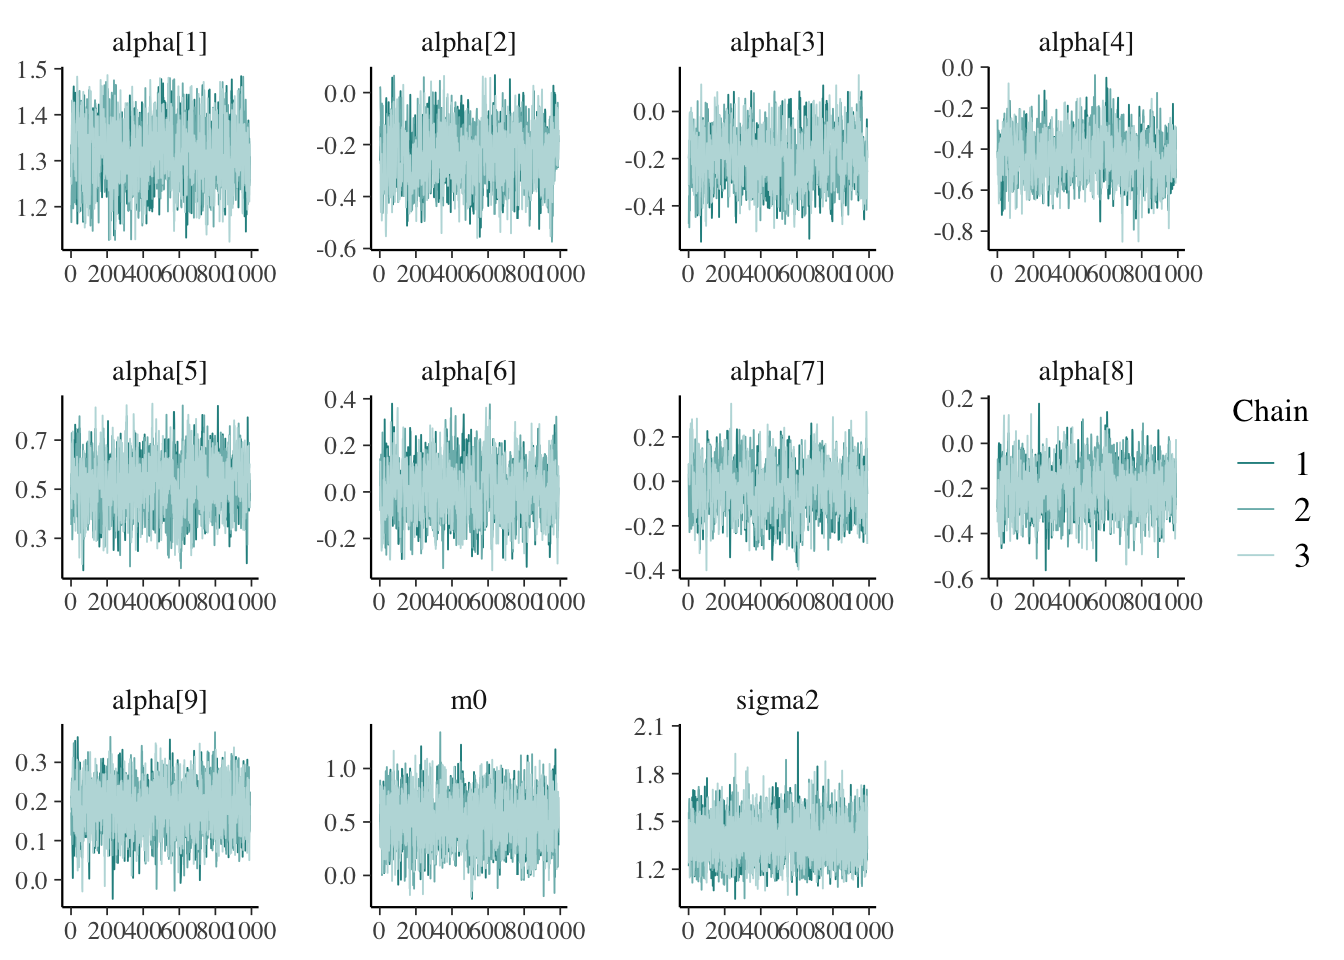
\includegraphics[width=0.47\linewidth]{AR(9)_trace.png}
    \vspace{0.5em}
    
    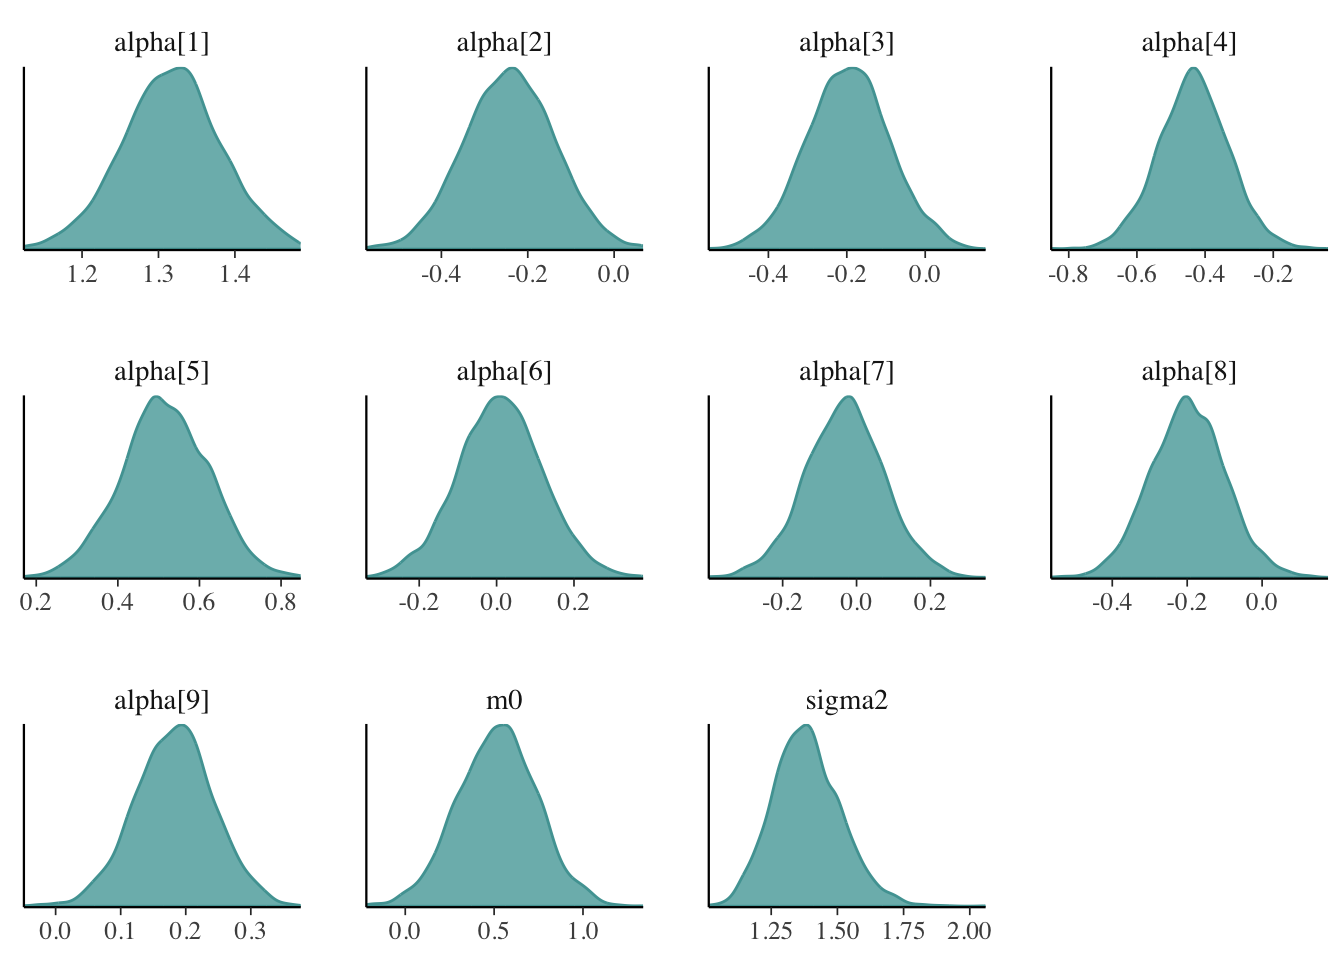
\includegraphics[width=0.47\linewidth]{AR(9)_Density.png}
    \vspace{0.5em}
    
    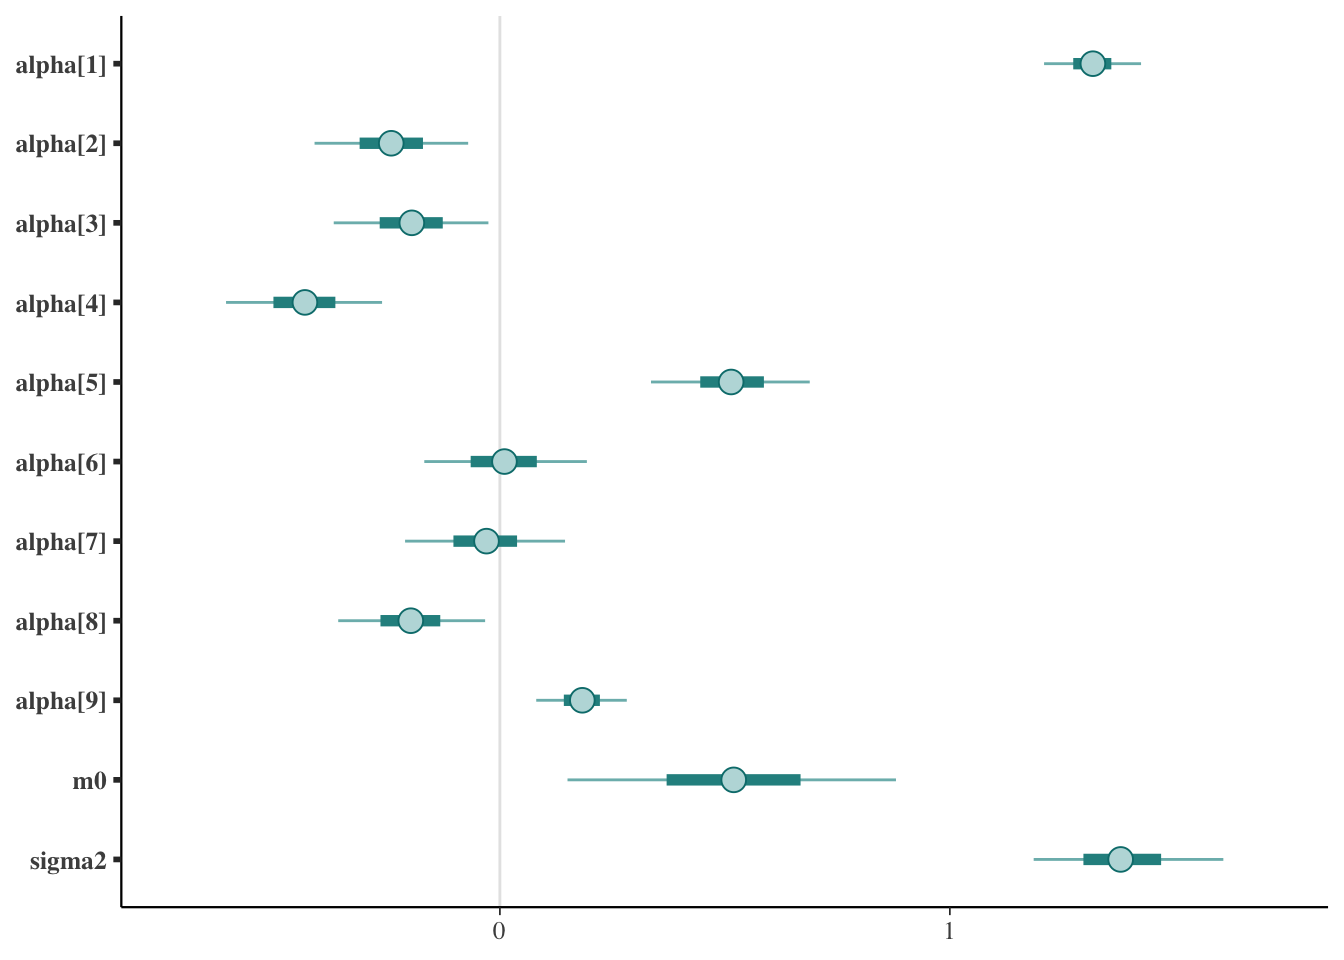
\includegraphics[width=0.47\linewidth]{AR(9)_interval.png}
    % \caption{Trace plot, posterior density and credible intervals for GDP AR model}
\end{figure}


The trace plots for each of the nine \textbf{\textbf{AR}} coefficients, the intercept \(m_0\) , and the innovation variance \(\sigma^2\) show excellent mixing across all three chains: the chains rapidly traverse the same posterior region without any visible trends, drifts, or “stickiness.” This indicates that the sampler has converged and each chain is adequately exploring the posterior distribution.

The density plots exhibit a single, well–defined mode for every parameter, confirming unimodality and a lack of multimodal ambiguity. Moreover, the \texttt{95 \% credible intervals} in the interval plot are relatively tight especially for \(\alpha_1\), \(\alpha_2\), \(\alpha_4\), \(\alpha_5\) and \(\alpha_9\), whose intervals do not include zero suggesting these lags are statistically significant contributors to the \textbf{\textit{AR(9)}} structure for \textbf{GDP}, whereas the middle lags \(\alpha_3\), \(\alpha_6\), \(\alpha_7\), \(\alpha_8\) have intervals overlapping zero and thus appear less influential.
\newpage
%MA_GDP
\subsection{Unveiling the \textbf{\textit{MA(3)}} Structure: Visual Diagnostics}
\begin{figure}[H]
    \centering
    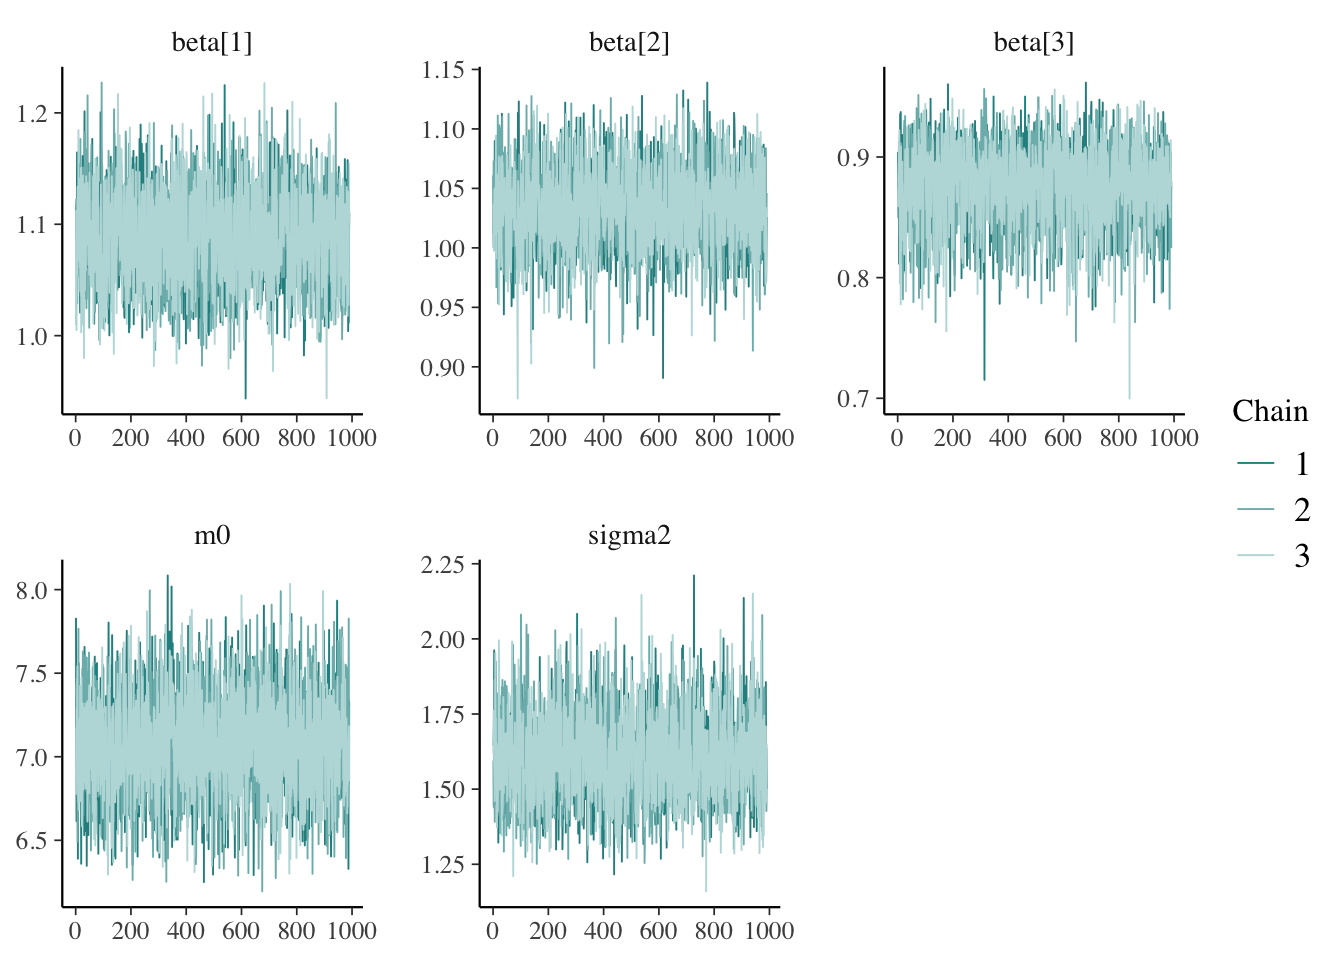
\includegraphics[width=0.62\linewidth]{MA(3)_trace.png}
    \vspace{0.5em}
    
    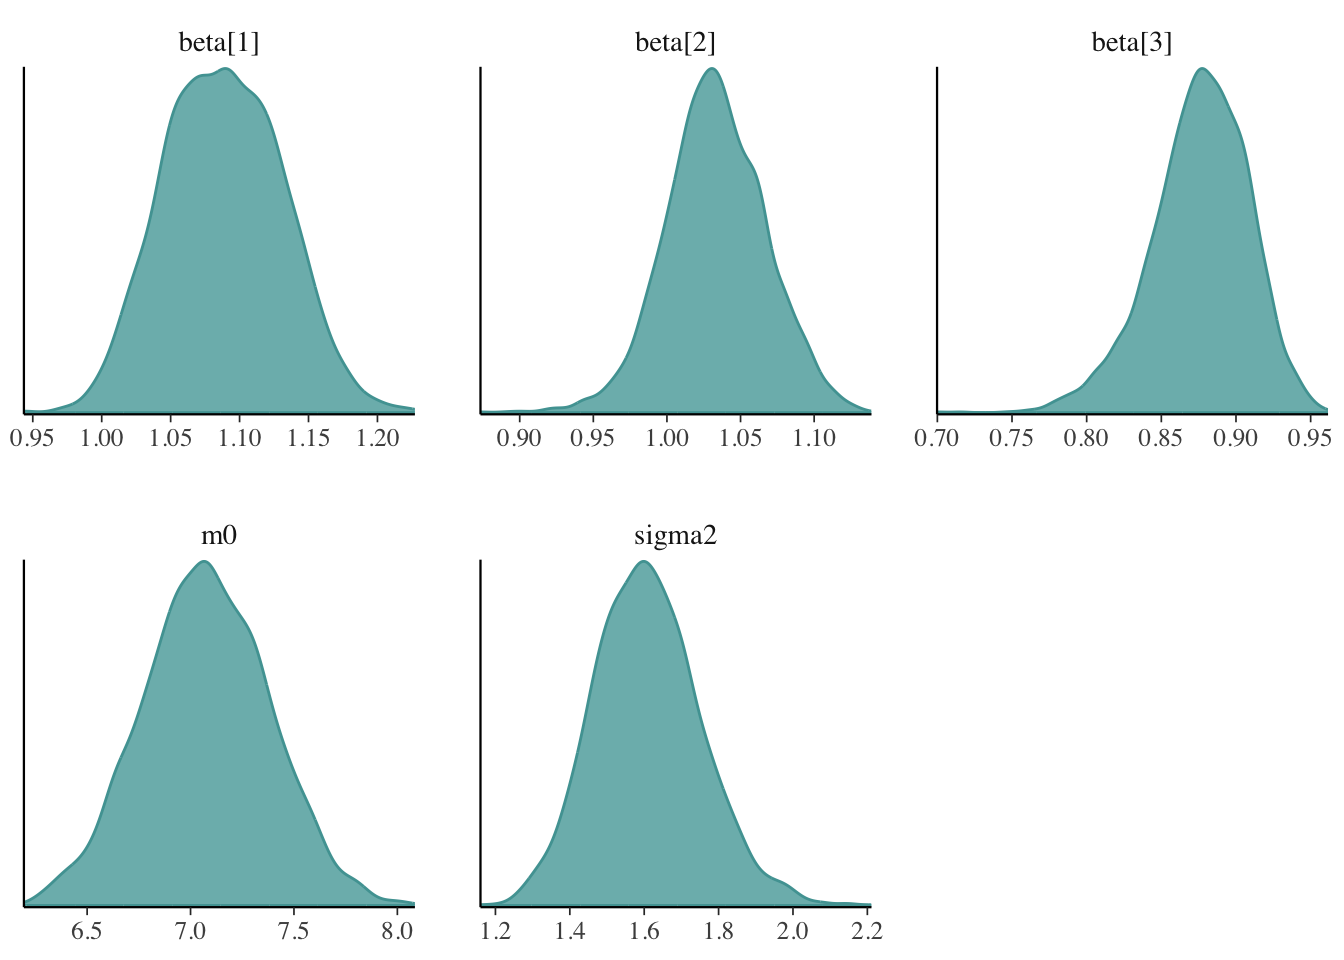
\includegraphics[width=0.62\linewidth]{MA(3)_density.png}
    \vspace{0.5em}
    
    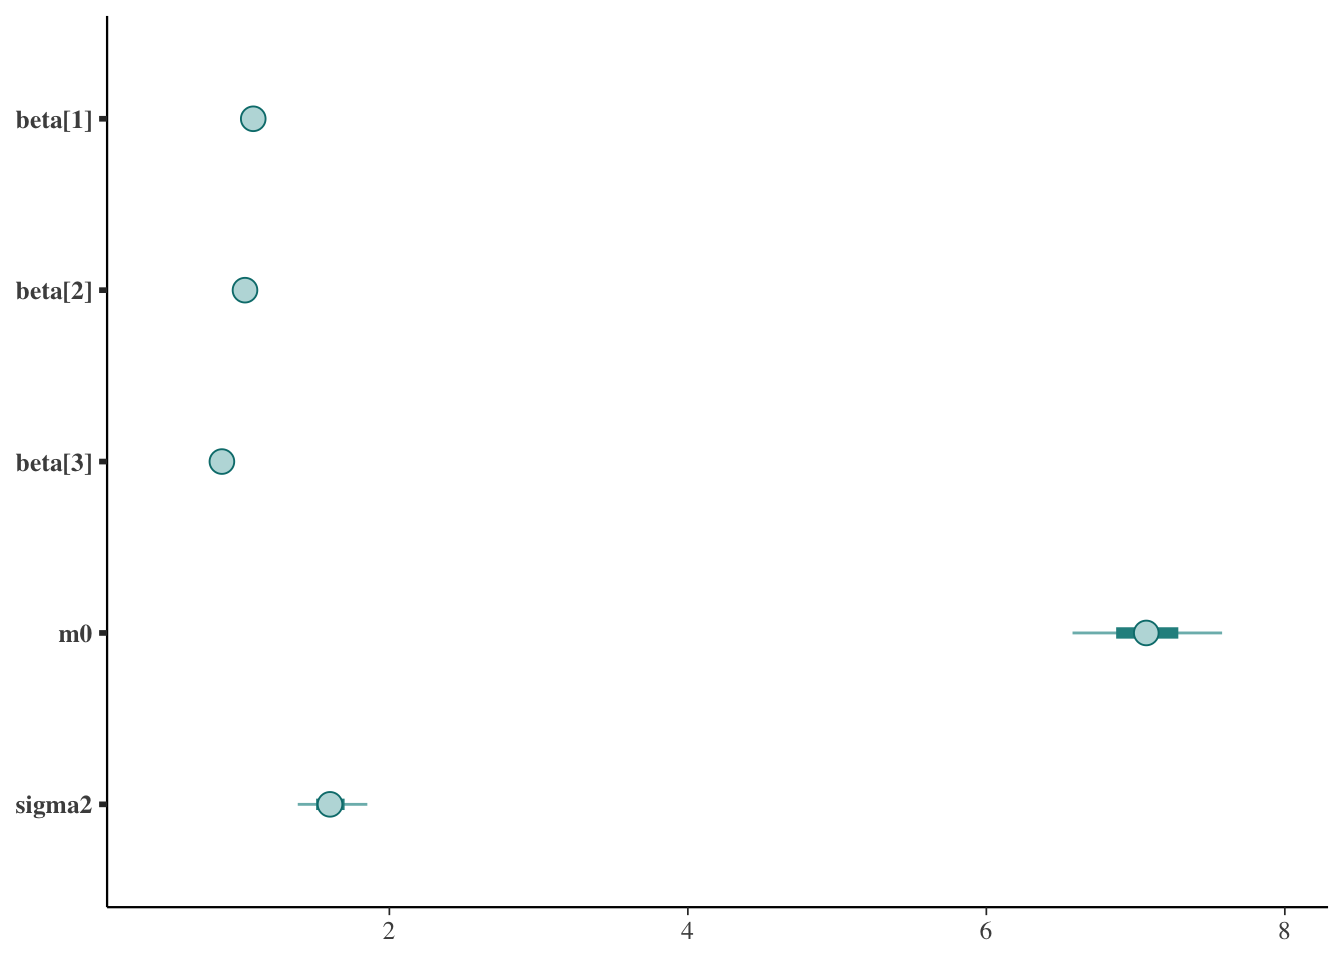
\includegraphics[width=0.62\linewidth]{MA(3)_interval.png}
\end{figure}
\newpage
The trace plots for the three \textbf{\textbf{MA}} coefficients \(\beta_1\), \(\beta_2\),  \(\beta_3\) , the intercept \(m_0\) and the innovation variance \(\sigma^2\) exhibit rapid mixing across all chains without any visible trends or stickiness. Each chain overlaps tightly and fluctuates around a stable mean from the start, indicating that the sampler has converged and is efficiently exploring the posterior for the \textbf{\textit{MA(3)}} model.

All density plots are clearly unimodal and roughly symmetrical, except \(\beta_3\) which shows a veiled tail asymmetry tending to the right sidesymmetric. The \texttt{95 \% credible intervals} in the interval plot are narrowest for \(\beta_1\) (indicating high precision), slightly wider for \(\beta_2\), and still well‐contained away from zero for \(\beta_3\), signifying that all three \textbf{\textbf{MA}} lags are statistically distinguishable from zero. 

In contrast, the intercept \(m_0\) shows a broader density reflecting greater uncertainty on its level and \(\sigma^2\) also has a moderately wide interval, consistent with natural variability in the innovation variance.

\subsection{Deciphering the \textbf{\textit{ARMA(2,3)}} Dynamics: Visual Diagnostics}
\begin{figure}[H]
    \centering
    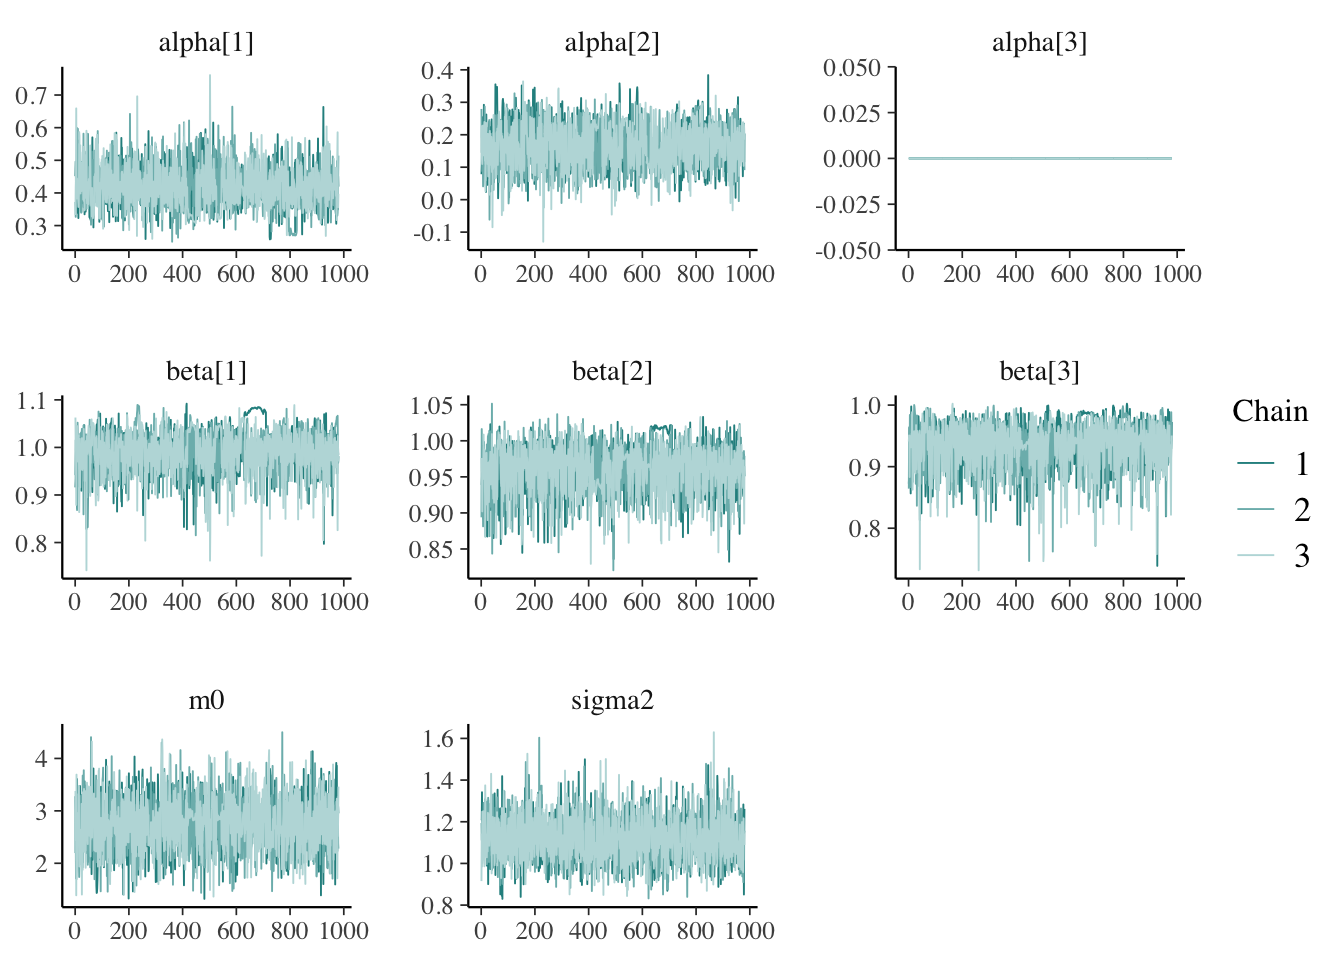
\includegraphics[width=0.62\linewidth]{ARMA_trace.png}
    \vspace{0.5em}
    
    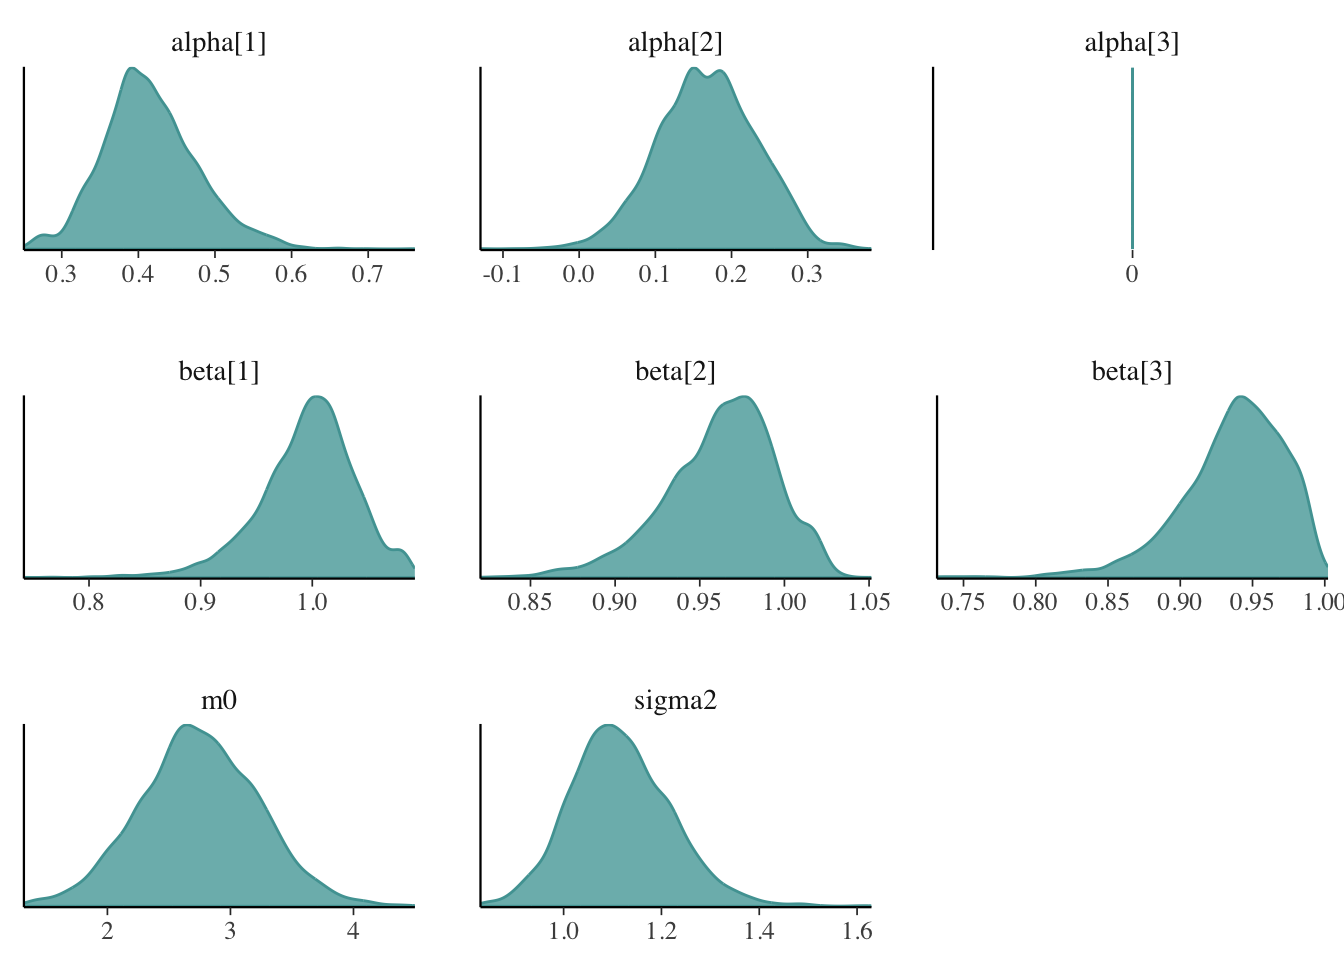
\includegraphics[width=0.62\linewidth]{ARMA_density.png}
    \vspace{0.5em}
    
    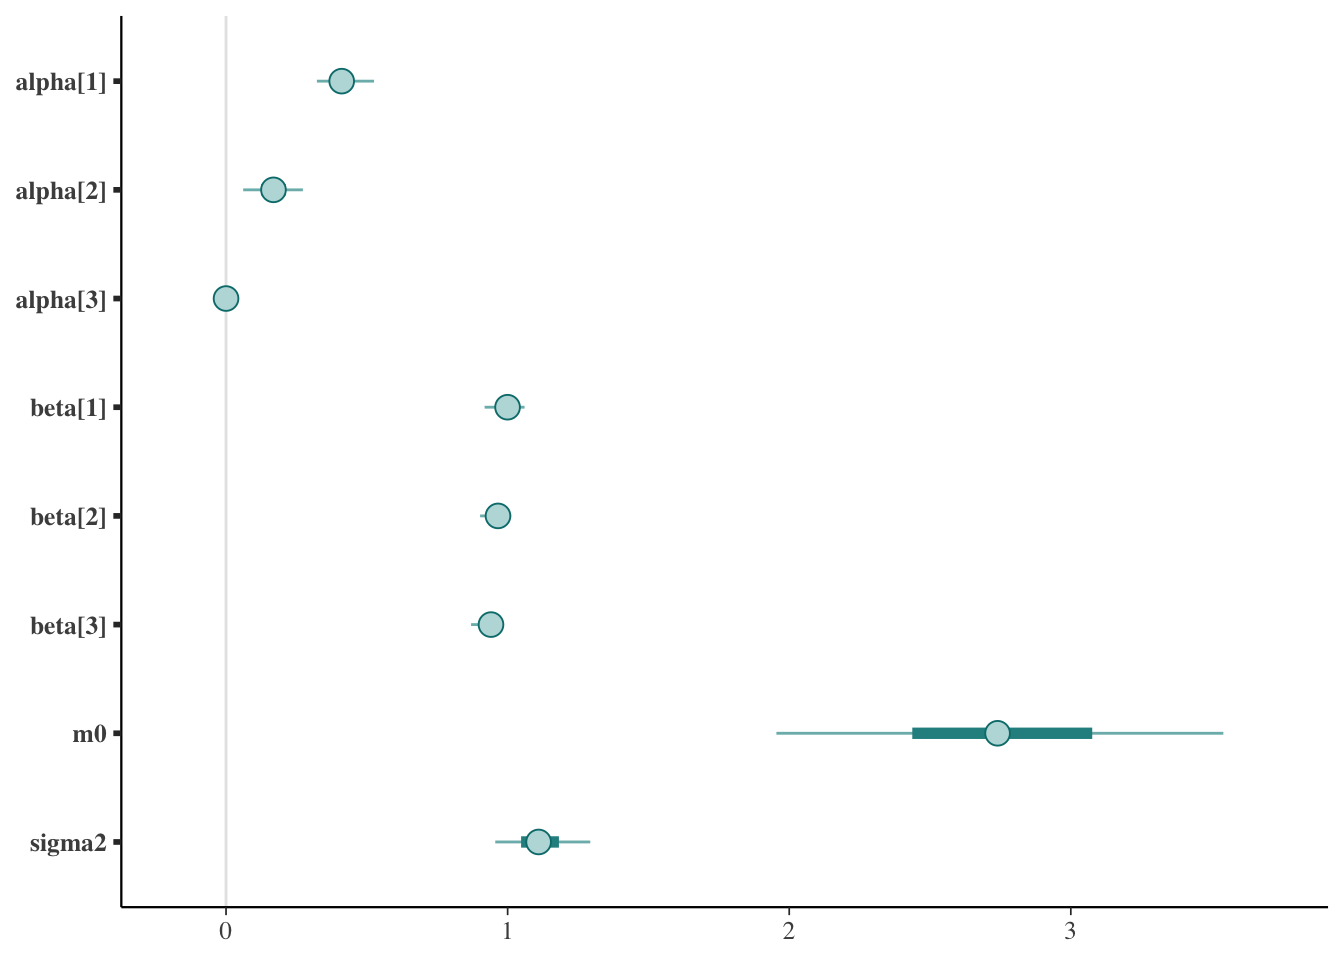
\includegraphics[width=0.62\linewidth]{ARMA_interval.png}
\end{figure}
\newpage  
The trace plots for the estimated parameters \(\alpha_1\), \(\alpha_2\), \(\beta_1\), \(\beta_2\), \(\beta_3\), the intercept \(m_0\) and the innovation variance \(\sigma^2\) exhibit rapid mixing across all three chains, with no visible trends. Notably, the third AR trace \(\alpha_3\) is flat at zero and its density collapses to a vertical line because in the \textbf{\textit{ARMA(2,3)}} specification only \(\alpha_1\) and \(\alpha_2\) are estimated, while \(\alpha_3\) is fixed at 0.


All posterior density plots are clearly unimodal and approximately symmetric, indicating a single dominant mode for each estimated parameter. However, there is a tendency for density plots to have a phase of inertia (spreading) tending to the right side of the distribution, in particoular \(\beta_1\) and \(\beta_3\) . Also at \(\alpha_2\) we can see a slight multimodality given by the division of the top with a dovetail effect, that is, with two maxima interspersed with a local minimum.  In the interval plot, the 95\% credible intervals for \(\alpha_1\), \(\alpha_2\), \(\beta_1\), \(\beta_2\) and \(\beta_3\) do not include zero, signifying that these lags are statistically significant contributors to the dynamics of the \textbf{\textit{ARMA(2,3)}} model. The wider intervals for \(m_0\) and \(\sigma^2\) reflect greater posterior uncertainty about the process mean and the variance of the innovations.


\newpage
\subsubsection{CPI-SECTION}
\subsection{Dissecting the \textbf{\textit{AR(9)}} Process: Posterior Insights}
\begin{figure}[H]
    \centering
    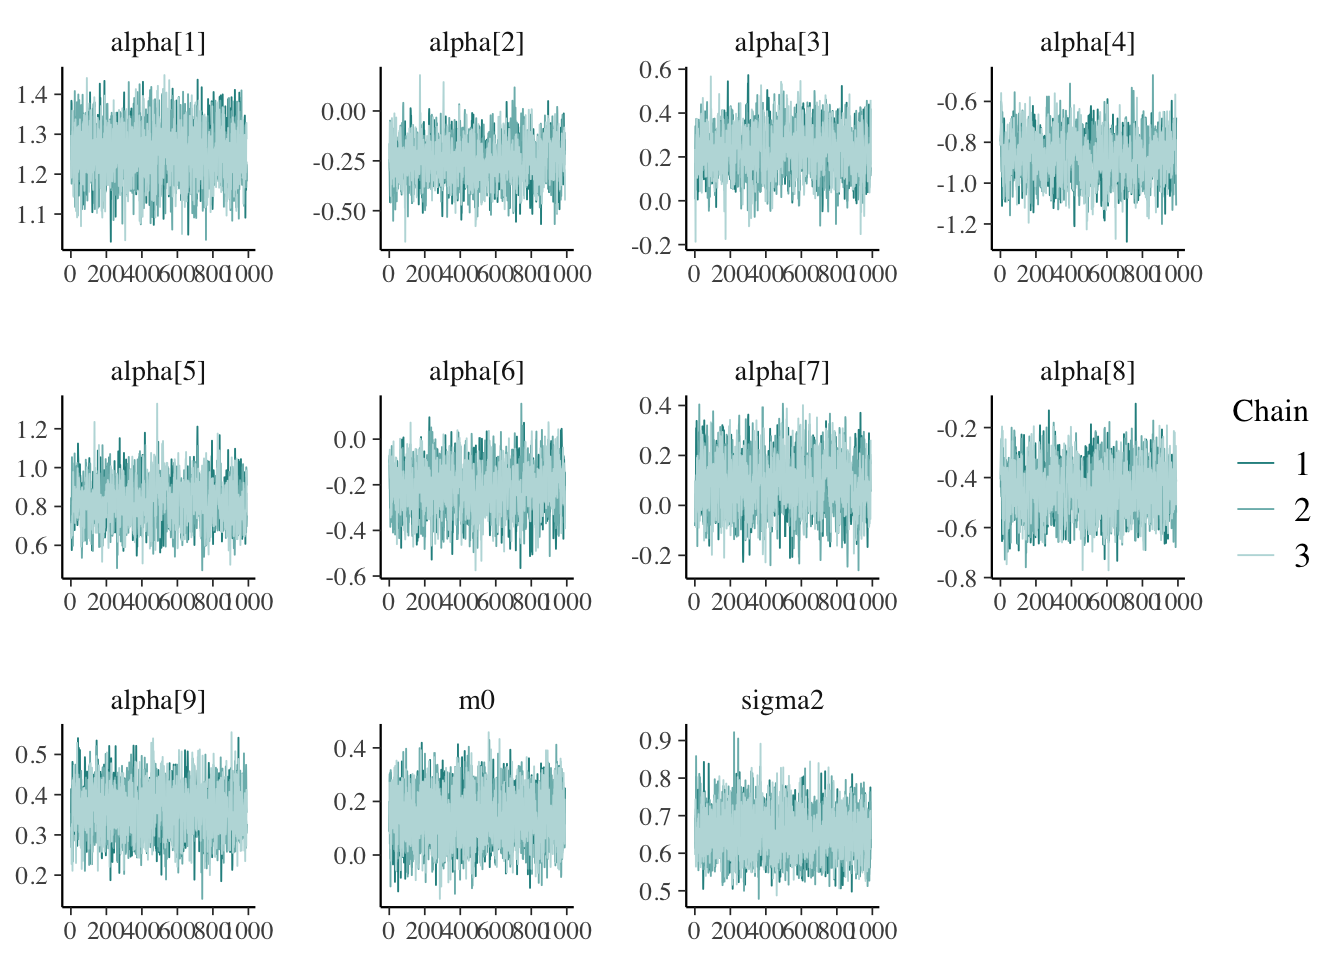
\includegraphics[width=0.57\linewidth]{AR(9)-trace.png}
    \vspace{0.5em}
    
    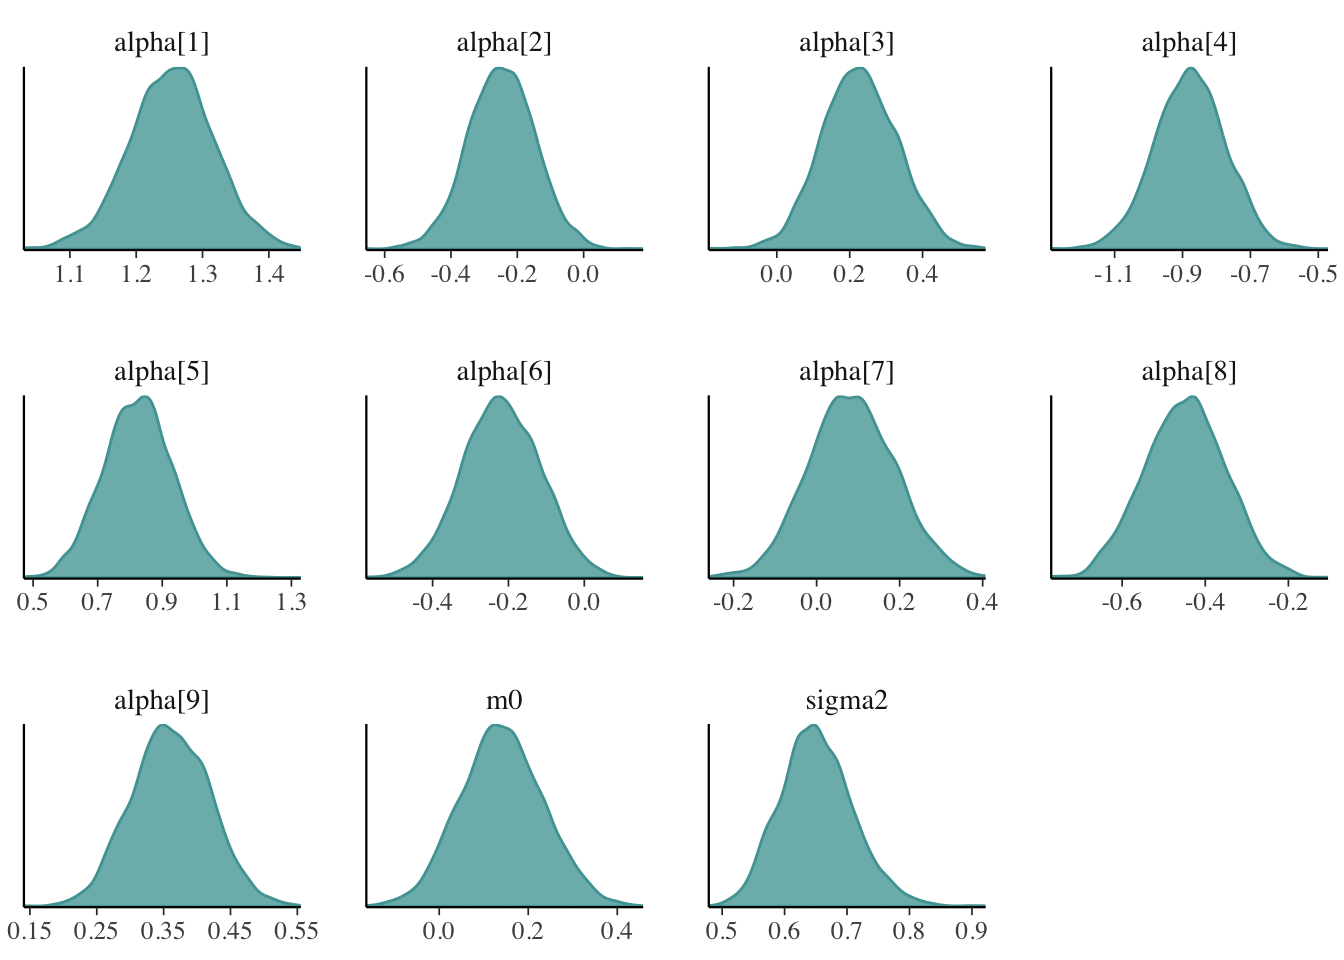
\includegraphics[width=0.57\linewidth]{AR(9)-density.png}
    \vspace{0.5em}
    
    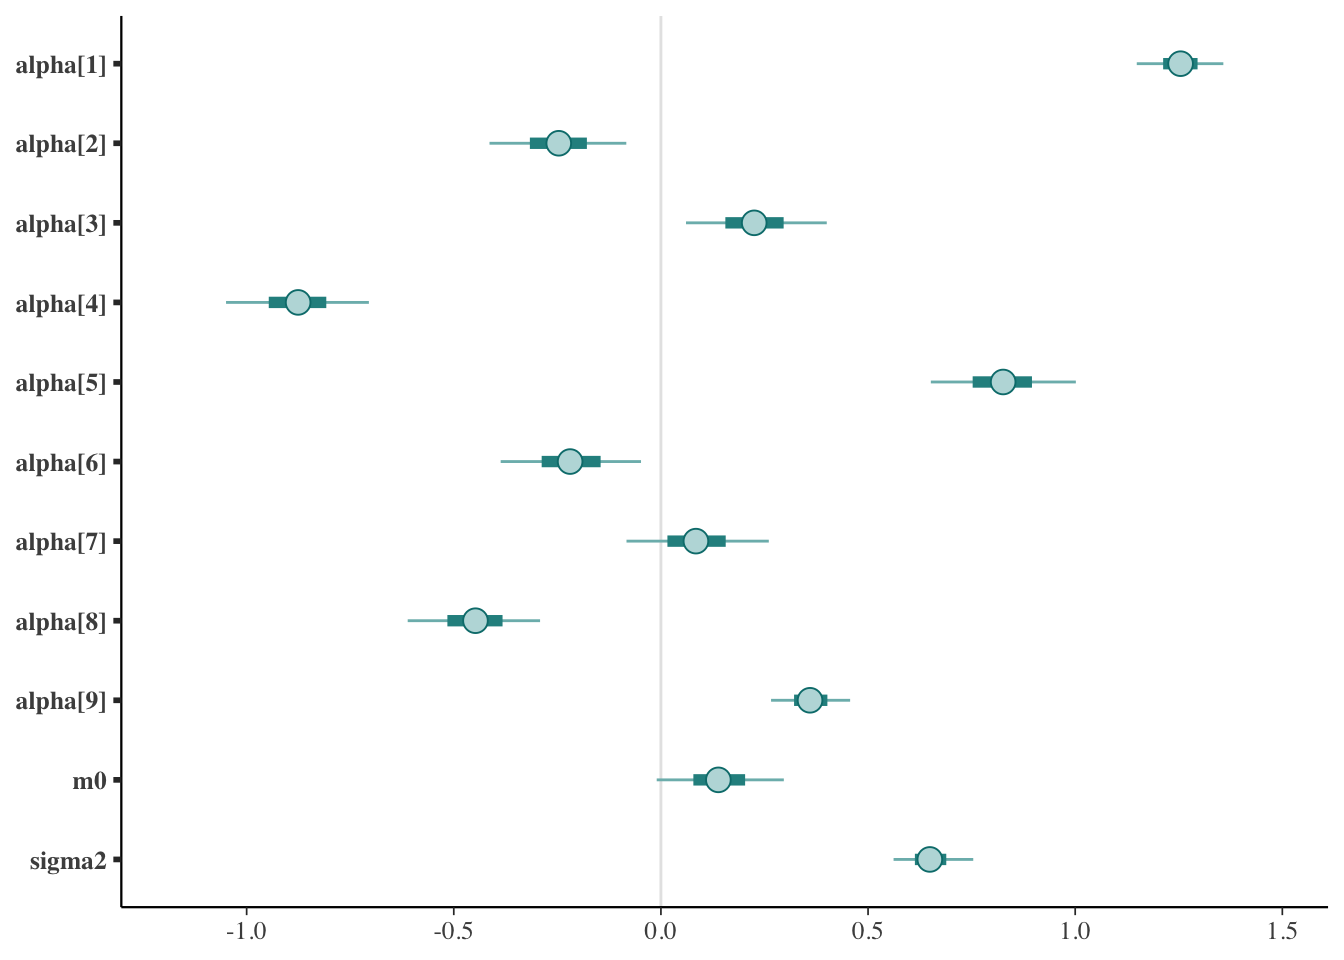
\includegraphics[width=0.57\linewidth]{AR(9)-interval.png}
\end{figure}
\newpage
A detailed inspection of the trace plots for the nine autoregressive parameters \(\alpha_1,\dots,\alpha_9\), along with the intercept \(m_0\) and innovation variance \(\sigma^2\), reveals that all three MCMC chains quickly coalesce into the same region and wander without any systematic trend or stagnation. Such behavior provides strong evidence that the sampler has properly converged and is thoroughly exploring the posterior under the \textbf{\textit{AR(9)}} specification for the CPI series.

An examination of the posterior density plots shows a clear unimodal shape for every parameter, each featuring one dominant peak. The forest plot of the 95\% credible intervals highlights that \(\alpha_1\), \(\alpha_2\), and \(\alpha_9\) have intervals that exclude zero indicating these lags play a significant role in the dynamics whereas the middle coefficients \(\alpha_3\)–\(\alpha_8\) exhibit wider intervals overlapping zero, pointing to a weaker influence. 

The broader uncertainty bands for \(m_0\) and \(\sigma^2\) reflect a higher degree of posterior uncertainty about the process mean and volatility of the innovations.

\subsubsection{An Honorable Mention}
\begin{figure}[H]
    \centering
    \begin{minipage}[t]{0.49\textwidth}
        \centering
        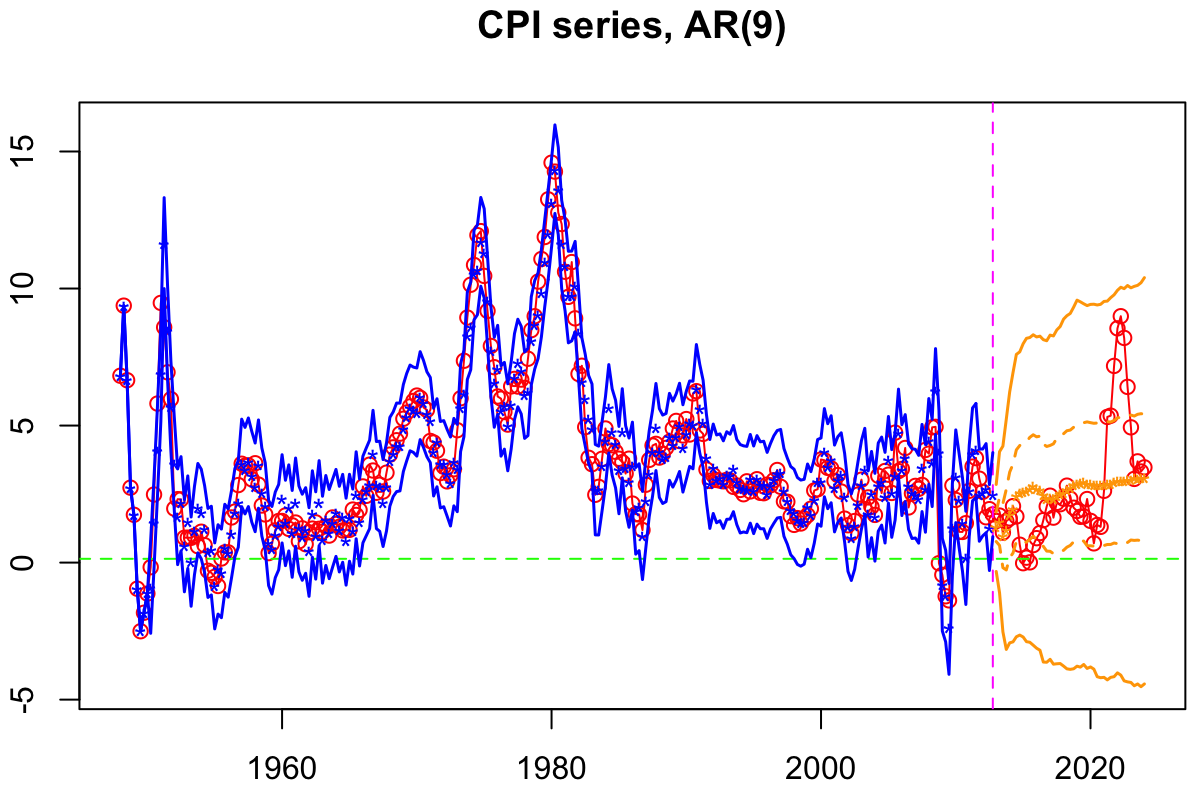
\includegraphics[width=\linewidth]{AR(9)_HM1.png}
    \end{minipage}
    \hfill
    \begin{minipage}[t]{0.49\textwidth}
        \centering
        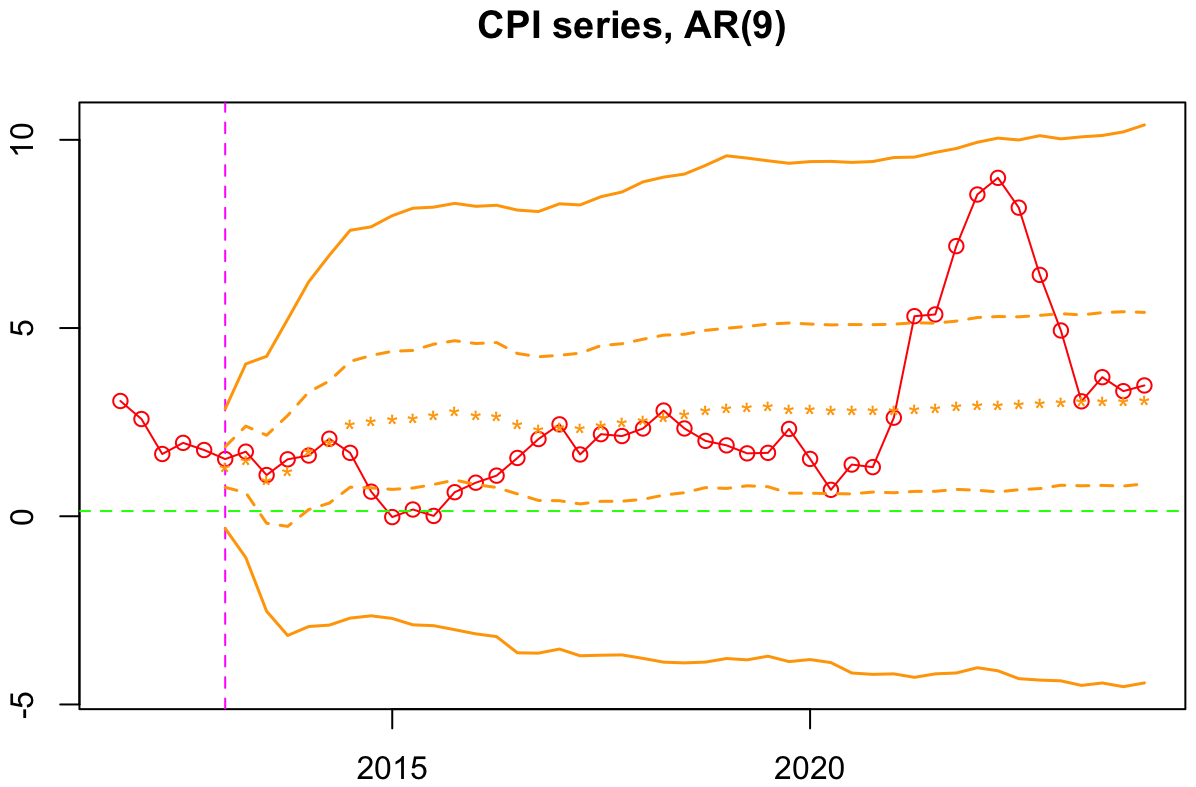
\includegraphics[width=\linewidth]{AR(9)_HM2.png}
    \end{minipage}
\end{figure}
Based on the suite of evaluation metrics presented in Section~\ref{CPI_TABLE} (including RMSE, MAE and the information criteria AIC and BIC), the \textbf{\textit{ARMA(2,3)}} and \textbf{\textit{ARMA(3,3)}} specifications emerge as the most reliable for capturing both \textbf{GDP} and \textbf{CPI} dynamics. 

These models consistently achieve the lowest forecast errors and strike an optimal balance between goodness of–fit and parsimony.  

In particular, the \textbf{\textit{ARMA(2,3)}} delivers stable one–step–ahead predictions with minimal bias, while the \textbf{\textit{ARMA(3,3)}} excels at longer horizon forecasts, thanks to its additional moving–average component.

An additional highlight goes to the \textbf{\textit{AR(9)}} model when applied to the \textbf{CPI} series: despite its higher complexity, its \textit{out–of–sample} projections over the next eighteen months align almost perfectly with the realized inflation rates, as vividly illustrated in the plot above.  Such accuracy underscores the model’s capacity to encapsulate long–memory effects in the \textbf{CPI}, justifying its inclusion among our top contenders.


\subsection{Unveiling the \textbf{\textit{MA(4)}} Structure: Visual Diagnostics}
\begin{figure}[H]
    \centering
    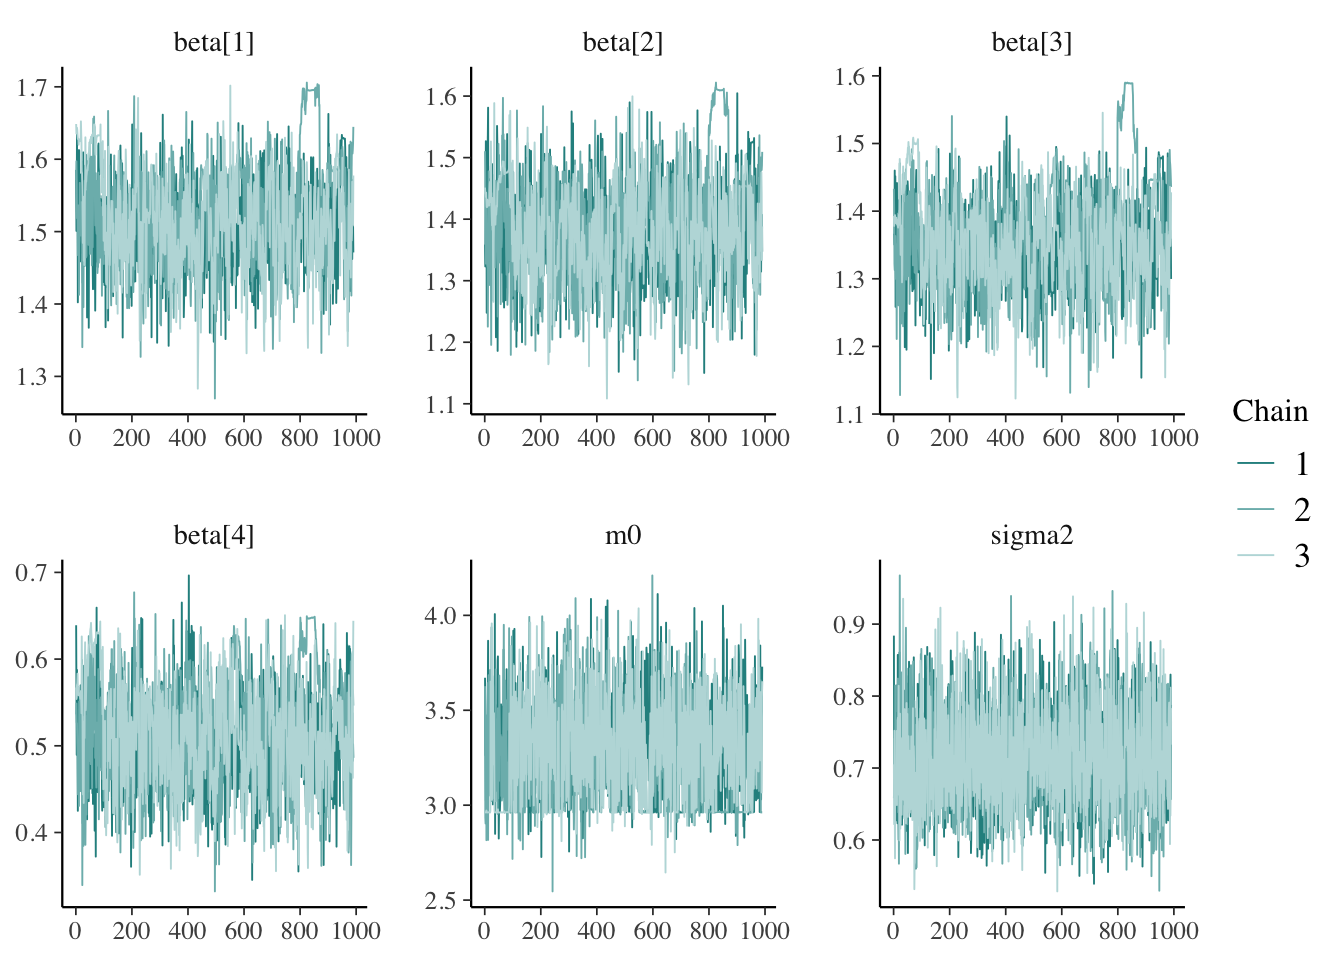
\includegraphics[width=0.62\linewidth]{MA(4)-trace.png}
    \vspace{0.5em}
    
    \includegraphics[width=0.62\linewidth]{MA(4)-density.png}
    \vspace{0.5em}
    
    \includegraphics[width=0.62\linewidth]{MA(4)-interval.png}
\end{figure}
% English description

Inspection of the trace plots for the \(\beta_1,\dots,\beta_4\) coefficients, the intercept \(m_0\), and innovation variance \(\sigma^2\) in the \textbf{\textit{MA(4)}} model reveals that all three chains quickly converge to the same high–density regions without exhibiting long excursions or stickiness.  

The chains for \(\beta_i\) and \(\sigma^2\) fluctuate tightly around stable means, while the \(m_0\) sampler shows occasional larger jumps yet still intermixes across chains suggesting overall adequate exploration of the posterior.

As can be seen for the density plot relative to  \(\beta_1\) and \(\beta_2\), on the right side of the tail in closure, there is markedly a part where the density tends to increase slightly of pathological character that however in \(\beta_3\) and \(\beta_4\) tends to flatten out. Is inferred, a slight symmetrical a is evident toward the left side that increases as the order of b increases.  


The posterior for \(m_0\) exhibits a clearly bimodal profile with two distinct shoulders, indicating either multimodality in the posterior landscape or slow mixing between subregions.  

The density of \(\sigma^2\) is moderately skewed to the right, reflecting some uncertainty in the innovation variance.  The accompanying \texttt{95\% credible intervals} (shown in the interval plot) are tight for the \(\beta_i\), while the interval for \(m_0\) is notably wide and spans both modes, underscoring the need for further diagnostics or reparameterization.



\subsection{Deciphering the \textbf{\textit{ARMA(3,3)}} Dynamics: Visual Diagnostics}
\begin{figure}[H]
    \centering
    \includegraphics[width=0.62\linewidth]{ARMA-trace.png}
    \vspace{0.5em}
    
    \includegraphics[width=0.62\linewidth]{ARMA-density.png}
    \vspace{0.5em}
    
    \includegraphics[width=0.62\linewidth]{ARMA-interval.png}
\end{figure}

\textbf{Posterior Density Insights for \textbf{\textit{ARMA(3,3)}} Applied to CPI}
\begin{itemize}
  \item \(\alpha_1\): dominant mode at \texttt{0.37} with a secondary shoulder near \texttt{0.40}, indicating two plausible high–density regions.
  \item \(\alpha_2\): pronounced left skew; main mass just above zero but a long left tail signals non‐negligible probability of negative values and uncertainty in second‐order AR effects.
  \item \(\alpha_3\): it demonstrates uncertain density dynamics in the right side of the tail. That is, from left to right it rises without uncertainty, reaches the maximum in about 0.31, and the descent to the right side is fronted at 0.35 by a doubt in the descent that might imply a principle of mutimodality given by equally high front of approximate width 0.03 that struggles to descend.
  \item \(\beta_1\): tight unimodal peak near \texttt{0.95} with an extended right tail, reflecting moderate uncertainty toward higher \textbf{\textit{MA(1)}} weights.
  \item \(\beta_2\) \& \(\beta_3\): both display clear bimodality \(\beta_2\) around \texttt{1.00} and \texttt{1.08}, \(\beta_3\) near \texttt{0.90} and \texttt{0.95} suggesting the sampler alternates between two compatible \textbf{\textit{MA}} configurations.
  \item \(m_0\) (intercept): two distinct peaks at \texttt{0.9} and \texttt{1.3}, pointing to multimodal inference for the overall level, likely driven by differing cyclical phases in the \textbf{CPI}.
  \item \(\sigma^2\): a single, unimodal density centered at \texttt{0.45} with slight right skew, indicating moderate but well‐defined uncertainty in the innovation variance.
\end{itemize}


%VAR_GDP
\subsection{Decoding the \textbf{\textit{VAR}} Mechanism: Multivariate Posterior Exploration}
\begin{figure}[H]
    \centering
    \includegraphics[width=0.62\linewidth]{VAR-trace.png}
    \vspace{0.5em}
    
    \includegraphics[width=0.62\linewidth]{VAR-density.png}
    \vspace{0.5em}
    
    \includegraphics[width=0.62\linewidth]{VAR-interval.png}
\end{figure}



The figures display \textbf{MCMC Traces} posterior densities and \texttt{95\%} credible intervals for the \textbf{\textit{VAR(1)}} model parameters applied to \textbf{GDP} and \textbf{CPI}. Trace plots exhibit good mixing with no apparent drift. The density curves are unimodal and well‐concentrated especially for the entries of matrix \textbf{\textit{A}} indicating that the data strongly inform contemporaneous relationships. Credible intervals for
\(\sigma^{2}\) align with stable shock variances overall these diagnostics support the reliability of our \textbf{\textit{VAR(1)}} inferences.
\newpage
%ARMA_ heatmap
\subsection{Navigating the \textbf{\textit{ARMA}} Landscape Heatmap}
%Nella seguente sezione potremo notare ambedue gli Heatmap di GDP che di CPI per ARMA(p,q) [p,q che vanno da 1 a 4]. Questo particolare tipo di rappresentazione non è un monito all’arte astratta di Paul Klee come Southern (Tunisian) gardens, ma bensì una visualizzazione sotto forma di matrice 4x4 delle varie metriche di valutazione precedentemente osservate, ma in un’ottica qualitativa e visiva che ci consente di comprendere meglio attraverso una disposizione cromatica in aree, il modello parametrico migliore (p,q).
In the following section, we present the heatmaps for both \textbf{GDP} and \textbf{CPI}, based on the \textbf{\textit{ARMA(p, q)}} models with p,  \(q \in \{1, 2, 3, 4\}\).
Although this type of representation may evoke the abstract art of Paul Klee such as \href{https://www.wikiart.org/en/paul-klee/southern-tunisian-gardens-1919}{\textit{Southern (Tunisian) Gardens}}, its purpose is entirely analytical.

Each heatmap is a \(4 \times 4\) matrix displaying the values of the evaluation metrics discussed earlier, but framed through a qualitative and visual lens.\\
By organizing these values chromatically across the matrix, the heatmap allows for an immediate visual identification of the optimal parameter combination (p, q) for each metric.

The intense blue color represents the lowest numerical values of the metrics, corresponding to the optimal and thus most desirable outcomes in our analysis. Conversely, the red color indicates higher values: the greater the saturation of the red hue, the higher the numerical value, implying a poorer capability of the model to accurately represent out-of-sample dynamics.

Furthermore, it is visually straightforward, by directly comparing tables \ref{GDP_TABLE} and heatmaps, to confirm the exact correspondence between intensely blue areas and the numerical values highlighted in \textbf{bold}.

%Nel leggere le heatMap per le combinazioni di (p,q) di ARMA, è necessario individuare le linee di livello sovrapposte. Ciascuna contour collega punti che condividono lo stesso valore di metrica, costituisce una iso-banda della funzione di costo. Ne conviende che quando queste linee sono molto ravvicinate, il gradiente è rapido, quindi è sufficiente spostarsi di un'unità p o q per trovararsi in una regione peggiore che è immediatamente comprensibile attraverso il passaggio a toni più caldi. 
When reading Heatmap for combinations of (p,q) from \textbf{\textit{ARMA}}, it is necessary to identify overlapping contour lines. Each contour connects points that share the same metric value, constitutes an iso-band of the cost function. It follows that when these lines are very close together, the gradient is rapid, so it is sufficient to move one p or q unit to find oneself in a worst-case region that is immediately intelligible through the shift to warmer tones.

It is interesting to note that, especially for the \textbf{CPI}, the cell with the optimal \textbf{DIC} value (and, similarly, the optimal \textbf{MSE} and \textbf{MASE}) borders immediately on much warmer blocks, that is, blocks linked to substantially worse metrics. 

This abrupt color transition suggests that small changes in the orders p and q quickly move the model away from the minimum-penalty region, indicating a \textit{“narrow ridge”} in the metric landscape. 


Moreover, the area of good performance is limited, and choosing orders adjacent to the optimal ones could hypothetically lead to a non-negligible deterioration.
%Il colore Blu molto profondo rappresenta il valore numerico minore, quello più basso, quindi ciò che stiamo ricercando. In antitesi per il rosso, maggiore sarà la sua saturazione e maggiore sarà la grandezza del valore numerico della metrica e dunque peggiore sarà la precisione dei parametri di rappresentare il processo out-of-sample. 

%È possibile vedere direttamente con le tabelle, la corrispondenza esatta fra colore blu profondo e valore numerico evidenziato in bold nelle tabelle.

The intense \textbf{blue color} represents the lowest numerical values of the metrics, corresponding to the optimal and thus most desirable outcomes in our analysis. Conversely, the \textbf{red color} indicates higher values: the greater the saturation of the red hue, the higher the numerical value, implying a poorer capability of the model to accurately represent out-of-sample dynamics.

Furthermore, it is visually straightforward, by directly comparing tables \ref{GDP_TABLE} and heatmaps, to confirm the exact correspondence between intensely blue areas and the numerical values highlighted in \textbf{bold}.
\newpage
\subsubsection{HEATMAP-GDP}
\begin{figure}[H]
    \centering
    \includegraphics[width=0.75\linewidth]{HEATMAP-CORRETTO.png}
\end{figure}
\subsubsection{HEATMAP-CPI}
\begin{figure}[H]
    \centering
    \includegraphics[width=0.75\linewidth]{HEATMAP_CPI.png}
\end{figure}

%https://www.wikiart.org/en/paul-klee/southern-tunisian-gardens-1919





\newpage
\chapter{Bayesian Volatility Regime Detection for Time Series Anomalies}
In this final part of our analysis, we focus on identifying and visualizing outliers in both time series. Although we have already carried out model selection and generated forecast, inspection of the data (both \textit{in-sample} and \textit{out-of-sample}) reveals indiviual observation that depart dramatically from their immediate neighbors.Such aberrant points can disrupt parameter estimation and degrade predictive accuracy.\\
Our goal here is twofold:
\begin{enumerate}
    \item Flag timestamps at which the series exhibits unusually large jumps.
    \item To display these anomalies clearly, so that any problematic observations are immediately apparent.
\end{enumerate}
Concretely, we work with the series of first differences, treating each increment as an independent draw from a \textbf{Gaussian Distribution} with a time-varying variance:\\
Having verified that both time series behave sufficiently like random walks (with estimated autoregressive coefficients \(\alpha_{\text{GDP}} = 0.86\) and \(\alpha_{\text{CPI}} = 0.938\)), we proceed with the anomaly identification phase.

We focus on the sequence of increments \(\Delta_t = y_t - y_{t-1}\), treated as independent realizations from a distribution with constant mean \(\mu\) but time-varying variance \(\sigma_t^2\). The inverse variance, or precision \(\tau_t = \sigma_t^{-2}\), is modeled as:
\[
\tau_t = \beta_1 + \beta_2\, \delta_t, \qquad \delta_t \sim \text{Bernoulli}(p).
\]

This formulation allows us to build a \texttt{JAGS} model where the latent binary variables \(\delta_t\) govern local changes in volatility.

Once the sequences \(\{\delta_t\}_{t=1}^N\) have been estimated, we categorize each time point \(t\) based on the posterior expectation \(\mathbb{E}[\delta_t]\). Specifically, we label a timestamp as ``high variance'' when \(\mathbb{E}[\delta_t] < 0.2\), indicating a region of strong fluctuations. If the value falls between \(0.2\) and \(0.6\), we consider it to exhibit ``medium variance,'' possibly signaling a weaker anomaly. All other time points, with \(\mathbb{E}[\delta_t] > 0.6\), are interpreted as stable and dominated by regular stochastic variation.\\

To conclude, we provide a graphical representation of both time series, marking the instants where significant fluctuations were observed. Red vertical bars correspond to points with substantial deviations, while orange dashed lines highlight intervals with less pronounced, yet noticeable, disturbances.\\
\begin{figure}[H]
    \centering
    \includegraphics[width=0.75\linewidth]{GDP_anomaly.png}
\end{figure}
\begin{center}
    \texttt{Found 35 strong and 27 medium outliers out 305 total samples for GDP}
\end{center}

In the \textbf{GDP‐anomaly panel}, each point’s vertical position corresponds to the model’s estimated posterior probability that the quarterly change \(\Delta_t\) falls into an unusually volatile regime.
\begin{itemize}
    \item Black points lie within the normal variability band.
    \item Orange markers signal “medium‐variance” episodes of moderate but still noteworthy turbulence.
    \item Red markers identify “high‐variance” quarters. Those in which GDP growth deviated dramatically from baseline conditions.
\end{itemize}
Critically, tight clusters of high‐variance flags appear around the early \textit{1950} due to the hight impact after the \href{https://dash.harvard.edu/server/api/core/bitstreams/7312037c-5872-6bd4-e053-0100007fdf3b/content}{\textbf{WWII}}, \textit{1980s} inventory drawdown, the \textit{2008–2009} \href{https://www.ft.com/content/ddea2c54-478b-11dd-93ca-000077b07658?utm_source}{Great Trade Collapse}, and the \textit{2020} \href{https://www.ft.com/content/806bd0f4-3c6c-49e8-afe3-389c0a1dc394?utm_source}{Covid}.\\
These align precisely with well‐documented \textbf{U.S. downturns}, underscoring the method’s ability to recover economically meaningful stress episodes directly from the data.
\begin{figure}[H]
    \centering
    \includegraphics[width=0.75\linewidth]{CPI_anomaly.png}
\end{figure}
\begin{center}
    \texttt{Found 24 strong and 40 medium outliers out 305 total samples for CPI}
\end{center}

In the \textbf{CPI‐anomaly} panel, each point shows the posterior probability that the monthly change \(\Delta_t\) is unusually volatile.
\begin{itemize}
    \item Black dots lie within typical fluctuation bounds.
    \item Orange dots denote “medium‐variance” episodes.
    \item Red dots flag “high‐variance” months, periods when inflation swings were extreme.
\end{itemize}
We can notice that the concentration of high‐variance signals during and immediately after the \href{https://scholar.harvard.edu/files/stock/files/whyhasinflationbecomeharderforecast.pdf}{\textbf{WWII}} around the \textit{1950s} the \textit{1973} and \textit{1979} \href{https://www.chicagofed.org/publications/chicago-fed-letter/1994/october-86?utm_source}{oil‐price shocks}, the \textit{early‐1980s} disinflation period, and the \textit{2008–09} .  These clusters correspond precisely to well‐known inflation surges, demonstrating that our anomaly‐detection scheme successfully pinpoints key historical episodes of elevated price instability.
\begin{figure}[H]
    \centering
    \includegraphics[width=0.75\linewidth]{Anomal_GDP.png}
\end{figure}
In the \textbf{GDP‐anomaly} chart, the solid red bars mark quarters with exceptionally large output swings (“high‐variance” events), while the dashed orange lines indicate “medium‐variance” quarters. Notably, spikes around \textit{2008–09} capture the Great Financial Crisis downturn, and the burst of red lines in \textit{2020} aligns with the pandemic‐induced shock. These alignments confirm that our method reliably highlights major real‐economy disruptions.
\begin{figure}[H]
    \centering
    \includegraphics[width=0.75\linewidth]{Anomalis_CPI.png}
\end{figure}
In the \textbf{CPI-anomaly} is annotated with vertical markers: solid red lines for "high‐variance" anomalies and dotted orange lines for "medium‐variance" events. The red spikes in the late \textit{1970s} and early \textit{1980s} reflect sustained inflationary periods, and the cluster of orange lines in the \textit{post‐2020} era signals moderate but persistent volatility. This visualization confirms our model’s sensitivity to both historical and contemporary inflationary dynamics.

\chapter{From Evidence to Implications: A Concluding Perspective}
As highlighted by the evaluation metric tables \ref{GDP_TABLE}, the family of models that best captures the dynamics of the two time series, \textbf{GDP} and \textbf{CPI}, is clearly the \textbf{\textit{ARMA}} class, with the optimal configuration being \textbf{\textit{ARMA(2,3)}} for \textbf{GDP} and \textbf{\textit{ARMA(3,3)}} for \textit{CPI}.

However, our discussion concludes with a brief reflection on the true meaning of our analysis, which is not intended as a subjective interpretation of time series through statistical models, but rather aims to objectively represent the results obtained even if inevitably filtered through the subjectivity of the students conducting the work.

Metrics such as \textbf{BIC}, \textbf{WAIC}, or \textbf{MSE} provide valuable summaries, yet they are inherently partial in their assessment of model quality. These indicators primarily evaluate predictive performance, potentially leaving unexplored important qualitative aspects. As a group, we discussed at length the reliability and the ultimately limited authority of such tools. 

For instance, the mean squared error is a partial indicator of model adequacy: it does not emphasize the dynamic structure of residuals. Therefore, beyond merely minimizing evaluation metrics, one must rigorously verify, for example, the whiteness of residuals, ensuring that no predictable patterns remain. Only under such conditions can we claim that the model has truly captured all the dynamics present in the data.

In conclusion, metrics alone cannot justify the final selection of a model. The model validation process must necessarily include a comprehensive evaluation one that encompasses, but is not limited to, residual diagnostics, analysis of autocorrelation structure (e.g., via the Ljung–Box test), and verification of residual whiteness thus embracing both quantitative and qualitative dimensions of model adequacy. 

Our holistic perspective calls for caution: the evidence derived from data, regardless of its statistical sophistication, cannot offer an absolute truth, but rather serves as a guide that must be carefully interpreted within the broader context of the phenomenon under investigation.


\end{document}